
\subsection{Fractional occupancy of BTA }
%\begin{equation}\label{}
%     f_{BTA} = w_{0} + \sum_{m} \left< n_{m} \right>|_{t}  w_{m}
%\end{equation}
%Here  $\left< n_{m} \right>|_{t}$ is the average number of bound morphogen m, where the expectation value is over the occupation time of the morphogen m to the CRM per nuclear cycle of synthesis (similar to the time elapsed between cell divisions, but flies do not have 'cells' in early development).  $w_{0}$ is the 'y intercept' and $w_{m}$ is the 'slope'.
\begin{figure}
  % Requires \usepackage{graphicx}
  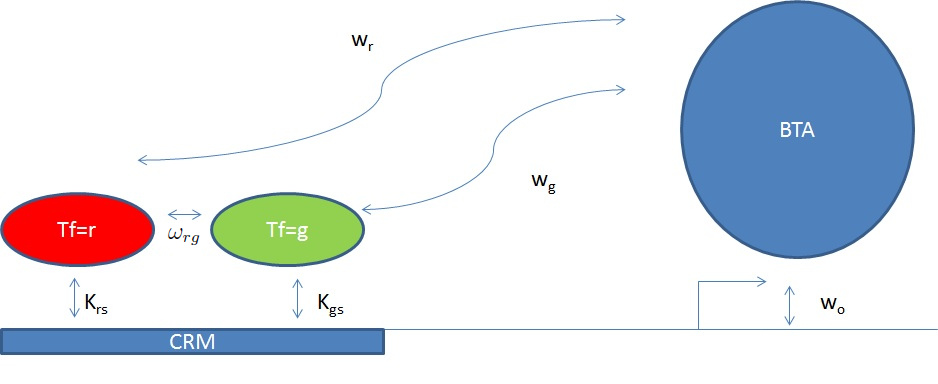
\includegraphics[width=1\textwidth]{PlugandPlay}\\
  \caption{Diagram of the components of fractional occupancy model, along with the parameters to bit through expression data (estimates of the mRNA output of the gene bound by the BTA and estimates of input morphogen concentrations).}\label{PlugandPlay}
\end{figure}

We can gain more physical insight into the problem by thinking of mechanisms of how BTA's occupancy is a function of the morphogen occupancy.  In Figure \ref{PlugandPlay} we see that when the morphogen's are bound they have an activation or repression domain, which communicates with the BTA, for our case this communication may be thought of as the complex process of changing the epigenitic state of the chromosome, by coactivators (histone modifiers, nucleosome remodelers) binding to the morphogen.  The binding energy of this domain ($w_m$) on the mophogen can be related to the binding energy of the BTA:
\begin{equation}\label{hilldg}
     \Delta G = w_{0} + \sum_{m}  n_m(c) w_{m}
\end{equation}
Here c is a particular configuration of the morphogens on the promoter, $w_0$ is the binding energy contribution from the basal promoter, $w_m$ is the binding energy contribution from each morphogen, and $n_m(c)$ is the number of bound morphogen of species m to state c (for example see \cite{pmid19956545}).  For this configuration we could model the occupancy of the BTA as:

\begin{equation}\label{segcon}
     f_{BTA}= \frac{1}{1 + e^{ -(w_{0} + \sum_{m}  n_m(c)   w_{m}})}
\end{equation}
The fast pace timing of morphogen binding relative to transcription time (e.g. the time for PolII to clear the promoter, and a new (or preloaded on the enhancer) PolII binds), would suggest that the BTA is not sampling or cognizant of each CRM configuration of bound proteins, rather the BTA sees an average occupancy of the morphogens.  This can be modeled as:
\begin{equation}\label{segcon2}
    f_{BTA}  = 1/(1 + \exp{ -(w_{0} + \sum_{m}  \  \left< n_m \right>|_{c} \ \ \ w_{m}) }),
\end{equation}
where the occupancy of the BTA is related to the theoretical model of average morphogen m occupancy over the CRM configurations $\left< n_m \right>|_{c}$\footnote{This can also be shown, under certain conditions, to be an approximation of the much more computationally intense model of Segal et.al\cite{pmid18172436} where they compute $ \left< f_{BTA} \right>|_c = \left<  \frac{1}{1 + e^{ -(w_{0} + \sum_{m}  n_m(c)   w_{m}})} \right>|_c$.  However, as stated above, this is not an approximation of Segal's model, it's a different model of the interaction of the BTA with the CRM.}.  The average morphogen occupancy over configurations is:
\begin{equation}
   \left< n_m \right>|_{c} = \sum_c n_m(c) \frac{W(c)}{\sum_c' W(c')},
   \end{equation}   
   where we the normalized weights of each configuration are from Equation\ref{mbody}, and $n_m(c) $, is the number of morphogen of type $m$ (such as $m=Dorsal$) bound to the configuration $c$.  The expectation value is computed using GEMSTAP software from Sinha's lab, see the following reference for further details\cite{pmid19956545}.  Here after, we simply use $ \left<n_m \right>$ to denote $\left< n_m \right>|_{c} $ with the understanding that the expectation value is taken over the binding configurations of the CRM. 
%However, there is also evidence that suggests PolII is seeing each configuration, such as CCC experiments that have sequenced enhancers captured at the promoter indicating the looping model which supports each configuration of bound morphogens contributing by using a model like Segals.

% an illustration of $<n_m>$ is given in the following slides:
%\includepdf[pages=-]{gropmeet1206ina.pdf}

\subsection{Fractional occupancy of BTA from a binding reaction perspective }
Let P = PolII concentration(this is the best known protein in the Basal Transcription Apparatus, but technically P is the concentration of the BTA), D = DNA (or basal promoter, i.e. TATA box, and binding sites for TF2B etc..), C = complex (PD).  We assume the binding process is in equilibrium (different timescale than morphogen binding).
\begin{equation}\label{}
    P + D \Leftrightarrow C
\end{equation}

Using fractional occupancy we have:
\begin{equation}\label{}
    \frac{C}{C + D} = \frac{1}{\frac{D}{C} + 1}
\end{equation}
\begin{equation}\label{}
    C = P*D*K_a
\end{equation}

\begin{equation}\label{}
   \frac{C}{C + D} = \frac{1}{\frac{D}{PDK_a} + 1} = \frac{1}{\frac{1}{PK_a} + 1}
\end{equation}
now assuming concentrations of unbound PolII is unaffected by our DNA D,we can say free PolII is a constant like 1000, and absorb the constant into the $K_a$,
\begin{equation}\label{rrr}
    \frac{1}{\frac{1}{PK_a} + 1} = \frac{1}{\frac{1}{K_a'} + 1} =\frac{1}{e^{-\frac{\Delta G}{k_bT} }+ 1}
\end{equation}
Now $\Delta G$ is the free energy that is released during morphogen binding, so  we can equate $ \Delta G $ to equation \eqref{hilldg}, however we will not say PolII 'sees' a particular configuration, rather we will assume PolII sees the average configuration (i.e. $<n_m>$ the average number of bound morphogen, m)
\begin{equation}\label{polenergy}
    \Delta G =  w_{0} + \sum_{m}  <n_m> w_{m}
\end{equation}

\begin{equation}\label{}
     <n_m> =\sum_c n_m(c) P(c)
     \end{equation}

plugging in the energy in units of $k_b T$  from equation \eqref{polenergy} into equation \eqref{rrr} we arrive again arrive at equation \eqref{segcon2}:
\begin{equation}\label{themodel}
      \frac{1}{\frac{1}{PK_a} + 1} = \frac{1}{e^{- (w_{0} + \sum_{m}  <n_m> w_{m} ) }+ 1}
\end{equation}

This yields a range of $N_{mRNA} \in [0,1]$.

\subsection{Fractional occupancy of BTA in Cooperative Binding (CB) model in Xin He's GEMSTAT}

The fractional occupancy in Xin He's Cooperative Binding model (CB) is closely analogous to our form of the model\footnote{This CB is not our related to our CB PWM model from chapter 2.}.  This can be seen by taking the simple system of one morphogen binding site with one basal promoter site for the BTA.  Hence, the BTA is treated as if it were simply another morphogen.  In this case the partition function of the two site system ($\Xi$) for the case that the two sites are independent is: $\Xi=(1+q)(1+q_{BTA})$, where q is the canonical partition function of the morphogen bound to its site and $q_{BTA}$ is the canonical partition function of the BTA bound to its promoter.  Now if we assume the sites are dependent, then we can not factorize the joint partition function\footnote{As always, we can \emph{organize} the states over our many-body system by systematically building the configurations, even in the case of dependencies, through a polynomial expansion over binding sites, which is presented in Xin He's Supplementary Material and T.Hill's text\cite{hill}.} and we then have $\Xi=(1+q+ q_{BTA} +q_{BTA} \ q \ w_{tf}) = Z_{off} + Z_{on}$, where we have collected similar terms in the expansion, where $Z_{off}=1+q$ is the term that does not include BTA binding, and $Z_off$ is the collection of the remaining terms (where BTA is bound)\footnote{In Xin's Supplement, $w_{tf}$ is denoted as $\alpha$ (which is a different parameter than our $\alpha$ that approximates the morphogen binding constant, where we choose the symbol $\alpha$ to mimic Segal's choice of parameters) $w_{tf}$ is the cooperative binding between the morphogen and the BTA}.  In their CB model they have $f_{BTA}=\frac{Z_{on}}{Z_{off}+Z_{on}}=\frac{1}{Z_{off}/Z_{on}+1}$.  By equating this to our form of the occupancy (Eq.\ref{themodel}) we have:
\begin{equation}
Z_{off}/Z_{on} = \exp{-w_o + \sum_{tf} w_{tf} < n >_{tf} }.
\end{equation}
The above equation is the odds \emph{for} BTA binding, hence the log odds is:
\begin{equation}
\ln{Z_{off}/Z_{on}} = -w_o + \sum_{tf} w_{tf} < n >_{tf} .
\end{equation}
Now, if we assume there is only one morphogen binding site, then the denominator of $< n >_{tf} $ is $Z_{off}$, and its numerator is q.  Hence we have:
\begin{equation}
\ln{\frac{(1+q)}{(q_{BTA} +q_{BTA} \ q \ w_{tf}')}} = -w_o +  w_{tf}\frac{q}{1+q},
\end{equation}
where we have replaced the Z's with their original q's and the $w_{tf}'$ denotes Xin's form of the cooperativity between BTA and morphogen (in order to distinguish from our cooperativity's symbol $w_{tf}$.  Using the properties of logarithms we can isolate $(1+q w_{tf}')$ from the left side of the equation, which leads to:
\begin{equation}
\ln{(1+q)} - \ln{q_{BTA}} - \ln{(1+qw_{tf}')} = -w_o +  w_{tf}\frac{q}{1+q},
\end{equation}
where $w_o$ is $\ln{q_{BTA}}$ leaving the result:
\begin{equation}
\ln{(1+q)} - \ln{(1+qw_{tf}')}=w_{tf}\frac{q}{1+q}
\end{equation}
rearranging we have:
\begin{equation}
(1+q)\ln{(1+q)} - (1+q)\ln{(1+qw_{tf}')}=w_{tf}{q}
\end{equation}
if q is less than one (morphogen has low concentration, for example), then the first term on the left is approximately zero, and if $w_{tf}'$ is not too large then to first order the Taylor expansion of $\ln(1+qw_{tf}')$ is -$qw_{tf}'$.  Hence it appears under this regime that Xin's CB model, with free parameters $\alpha$ are equivalent to our w factors.

\subsection{Fractional occupancy of BTA in Ay's model}

The fractional occupancy model in Fakhouri et.al.\cite{pmid20087339}, which we'll call Ay's model is similar to Segal's model, and hence similar to our form of the BTA occupancy\footnote{A distinguishing characteristic between Segal and Ay's work was that Ay's model contained high quality expression data (with error bars)\cite{}, while the input expression data to Segal's model was a boolean based 'on' 'off' data, which was smoothed (for example by using cubic splines).  Furthermore Segal's CRM input was just the sequences and PWMs of the morphogens regulating the CRMs (where the binding sites were to be 'discovered' using a PWM annotation model), while Ay's model knew exactly where the binding sites were within the CRMs, thereby not being hampered by false postive binding sites from PWM prediction of sites such as in Segal's arpproach.  Once Segal's model had annotated a CRM with the morphogen binding sites, his model and Ay's model, we aim to show in this section, were identical (assuming the annotation had no false negatives and false positives).}.  In Ay's model the probability of each configuration is an element in a vector of probabilities, where the vector is labeled \textbf{F} (where $\sum_c F_c =1$, where c encodes the binding configurations as the component index to the vector.).  Similar to Segal's model, each configuration causes a particular occupancy of the BTA, where the occupancy of the BTA for each configuration is a component of a vector $\rm \textbf{T}$.  Hence $ \rm \bm{T} \bullet \rm \bm{F} = \sum_c F_c T_c $ (which given one knows all the configurations, this is then very similar in form to Segal's model $<\frac{1}{1+e^{f(c)}}> \approx < T_c >$, where the expectation is taken over the binding configurations and $f(c)$ is Segal's function of each configuration.

A departure from Ay's model and our model is the quenching function that he denotes as $q(d)$, where d is the spacer distance in base pairs between the repressor and the activator.  Their model, like ours, bins the spacer distances to form the queching function (q is a piecewise defined function over the different intervals of spacing between the repressor and activator)\footnote{  (In the case of multiple repressor types, one would have a notation such as: $q(d)_{tf}$, where each repressor type has its own quenching function, or possibly just one universal quenching function, if all repressors ended up behaving the same.  What a discovery that would be!) }.  In his model each interval has a free parameter to be trained, which is analogous to our form of the pairwise potential for repression, for example $\omega_{Sn,Dl}(d)$ (the repression pair-wise potential between Snail and Dorsal), which is also a binned pair-wise potential in the same form.  However, the parameters depart in that our $\omega$'s occur in the partition function just as in Segal's model, while Ay's quenching parameters do not.  His quenching parameter goes back to a model form from John Reinitz(\cite{perplexus}), where quenching modulates the probability of configurations bound by the repressing transcription factors.  In this model modulate means that the $p=1$ norm of their probability vector $ ||F|| = \sum_c F_c^{p}=\sum_c F_c$ is a function of the amount of repression\footnote{The norm of the vector here is not a standard vector norm, rather it is a $p=1$ norm in mathematics, where the $p$ norm is defined as $||x|=|\sum_i x_i^{p}$. }. 

 For example, a module responding to activators under high concentrations, but with very low concentrations of repressor (making the Boltzmann weights of repression configurations zero) has the usual norm $\sum_c T_c=1$, while if the conditions are favorable for repression, (such as both high concentrations of repressors and activators AND a very strong repression pairwise potential), then if the q(d) function is large (its largest value is 'one') for the spacer distances d that occur between the activators and the repressors, then configurations with bound repressors have their probabilities modulated by factors of $(1-q(d))$ for each bound repressor, where d is the spacer between each repressor and its nearest neighbor (while there were other forms, or schemes, tested for this function rather than just nearest neighbors).  
 
 For example, for a module with 5 activator binding sites and 5 repressor binding sites (with no sites overlapping), then for the configuration with all binding sites bound, and each activator had a nearest neighbor bound repressor with a spacer at d=10 bp, then the Boltzmann probability of the all bound configuration is modulated by a factor $(1-q(d=10))^{5}$, and the result of this is: $F_c'(1-q(d=10))^{5}$, where c' is the configuration with all 10 sites bound\footnote{In Ay's model, the configuration vector c takes a similar form to our configuration vector, for example, Ay's representation of the example configuratin with 10 bound sites is $c'=[ARARARARAR]$, where A is for activator and R is for repressor.  This is a compact representation of our configuration vector in Figure\ref{configurationMatrixI}, compact in the sense that our configuration vector also displays information about the spacers and internal positions of a binding site (a 'silent' state)).}
 
The difference between Ay's model of quenching and ours is due to the quenching parameters (function) not occurring in the partition function.  Here we see if it is possible to \emph{equate} Ay's model form $\sum_c F_c T_c$ to Segal's model.  First let the occupancy function of the BTA, which is a function of the configuration, be denoted as:
 \begin{equation}
 T(x)=\frac{1-q}{1+exp{(-x)}}
 \end{equation}
 where q is the quenching efficiency from Ay's model, and x is a function of the binding configuration.  Ay's exact form was:
 \begin{equation}
 T'(x)=\frac{1}{1+\exp{(5-x)}},
 \end{equation} 
which we wish to adorn with the factors (1-q) (the probability modulation factors that contain the quenching parameter q), which will then allow the BTA occupancy to be modulated, thereby keeping the Boltzmann distribution over the binding configurations unperturbed by repressor morphogen binding.  Now, make a change of variables, let $(1-q)=e^{+w}$, where the symbol w has no particular meaning other than to capture the change of form in the expression.  Now we have:
\begin{equation}
 T(x)=\frac{\exp{+w}}{1+\exp{(-x)}},
 \end{equation}
 whereupon bringing the numerator's factor into the denominator we have:
 \begin{equation}
 T(x)=\frac{1}{\exp{(-w)}+\exp{(-x)}\exp{(-w)}},
 \end{equation}
Now we simply want this denominator to be of the form $1+\exp{(-x')}$, which would allow Ay's model to be expressed exactly in the same form as Segals.  Hence we again make the change of variables:
\begin{equation}
 \exp{(-w)}+\exp{(-x)}\exp{(-w)}=1+\exp{(-x')},
 \end{equation} 
 which leads to:
 \begin{equation}
 -x' = ln(\exp{(-x)} +q ) - \ln{(1-q)} 
 \end{equation}
 Hence we have:
 \begin{equation}
 T(x) = \frac{1}{1+ \frac{\exp{(-x)}+q}{1-q}}
 \end{equation}
 Now, it appears that the odds for BTA occupancy from Ay's model: $\frac{\exp{(-x)}+q}{(1-q)}$ must be equal to the odds for BTA occupancy from Segal's model: $e^{f(c)}$.  Setting the log odds equal to each other may allow for some deduction on what certain parameters 'mean' in terms of the two models, which would then be able to be traced to our model.
 \section{Data set }

We would like to know the key biochemical parameters that are utilized by Dorsal, Twist, and Snail as they regulate the genes that pattern the Dorsal Ventral axis of early development by producing expression profiles, a list of mRNA counts for each position along the DV axis.  Under standard nonlinear regression, one could imagine an experiment where one measures the response (the dependent variable) to systematic variations of the inputs (independent variables), these measurements can then be used to fit a nonlinear regression model, where the fit parameters are our biochemical parameters (such as the binding constants).  Here the response, is the gene expression levels, and the inputs are the morphogen and CRM information (described further in the data section).  This is a massive amount of experimentation in order to fit a nonlinear model.  However, following the interpretation of Segal et.al.\cite{pmid18172436}, which in a sense, is a reinterpretation of Ed Lewis' model of homeogenes, and further refined by Zinzen et al.\cite{pmid16750631}, we can treat \emph{coordinately regulated} genes as if they were the \emph{same} gene, just under different inputs.  

What are the different inputs? The CRMs and positional information of the embryo (in terms of morphogen concentrations).  

How is this possible?  During development morphogens work together to coordinately regulate a set of genes.  

What about replicates, as a well designed experiment has statistical \emph{power}?  The number of degrees of freedom, which determines the statistical power, can be assumed infinite, as across a population of embryos, each with thousands of nuclei that each have a genome, we know the genome's are identical (neglecting short term evolution and segregation of SNPs during sex, where, SNPs in inbreed lab lineages is irrelevant.).  Each embryo is effectively a clone of one another.  

So, for the regulatory regions of genes, a modeler only effectively needs one sample to have complete knowledge about the DNA sequence, but what about the \emph{trans} enviroment, the numbers of each molecules in each embryo, doesn't that vary across embryos?  All embryo's are the same within limits of diffusion processes.  Each embryo across a population of embryo's is producing mRNA at each coordinately regulated gene with a high degree of precision.  Morphogen concentration gradients and the gene's expression response (mRNA levels) \emph{are} highly reproducible across different embryos, within the physical limits set by diffusion processes\cite{pmid17632062}.  So yes, the internal molecular environment from one embryo to the next does vary due to random walks of molecules.  However, our error in assuming that a population of embryos are all the same will be no bigger that $\sqrt{n}$, where $n$ is absolute number of a molecule type in each cell of an embryo.  Furthermore, $n(t)$, where $t$ is time, varies on a time scale much slower than the processes we will study.  Hence the \emph{diffusing} concentraition function across the embryo $n(z,t)$ where z is space (the DV axis), we assume is frozen.  For large $n$, the fractional error that we incur in our model is quite small.  Hence, variation in molecule in absolute concentration from one embryo to the next (or even within an embryo from one cell to the next cell - at the same position along the DV axis) is negligible.

Hence, we will treat an entire network of regulatory sequences as if they are each just a different measurement, a different input to our model.  This is a reasonable interpretation, however, nonlinear models are notorious to being sensitive in certain intervals of the input variables, and hence if the network has not just happened to evolve to coordiantely expressed gene's in the input regions where our model is sensitive, the model will fail, and one must resort to the tedious work such as Fukouri et.al.\cite{pmid20087339} to assure that all necessary data points are being collected (e.g. if one wants to measure distance dependent quenching, then one, under Segal's interpretation, should hope that evolution has selected a range of different spacers that coordinate quenching within the CRMs, otherwise the model fitting will be insensitive to this parameter.  Why?  Because there simply is no input data that varies the spacing, which is a prerequisite for fitting distance dependent interactions.).  However, the key biochemical parameters we are interested in was motivated by previous experiments of endogenous CRMs that have pointed to our parameters of interest of being the major contributing factors.  
%
%Since the coopertivity parameters are intricately linked with distance it makes sense to consider the distance between sites as the data as opposed the Sequence of the module (of course along with the binding site sequence information).
%  \begin{equation}\label{}
%        \mathbf{D}=\{\textbf{d}_t^{crm},\textbf{E}_t,\textbf{W}_t,\textbf{E}_{tf},\textbf{W}_{tf},\textbf{bs}_{tf}^{crm}\}
%    \end{equation}
%Where D is the same data set as in eqref, except now we have a set of separation distances and a set of binding sites (bs) for each module, as opposed to the module sequence and pwm.  the pwm is still useful here to give different weights to different sites within the module, although it would be interesting to know what is the variance in binding site affinity within a module given the threshold and pwm score used.
The model requires three main pieces of data denoted as $ \mathbf{D}$.  First, the CRM sequences and PWMs of the morphogen's targeting the sequences. Second, the morphogen concentrations along the DV axis at a particular point in time in development.  Third, the response of the CRM's to the morphogens (also in the form of 'expression' concentrations along the DV axis at a particular point in time in development). 


  \begin{equation}\label{datasetf}
        \mathbf{D}=\{\mathcal{S}_t^{crm},\mathcal{E}_t,\mathcal{E}_{tf},\textbf{PWM}_{tf} \}
    \end{equation}

\[
 \mathcal{S}_t^{crm}   =   \begin{pmatrix}

                      s_{rho}(1) & \ldots & s_{rho}(L_{rho})  \\
                      	 s_{vnd}(1) & \ldots & s_{vnd}(L_{vnd})  \\
                         \vdots & \ddots & \vdots   \\
                         s_n(1) & \ldots & s_n(L_n) 
                        \end{pmatrix}  =\begin{pmatrix}

                         % \hline
                          % after \\: \hline or \cline{col1-col2} \cline{col3-col4} ...
                          \textbf{S}_{rho}  \\
                          \textbf{S}_{vnd}  \\
                           \vdots \\
                         \textbf{S}_n 
                         % \hline
                        \end{pmatrix} \]
                       
                        \[
  \mathcal{E}_{t}  = \begin{pmatrix}
                         % \hline
                          % after \\: \hline or \cline{col1-col2} \cline{col3-col4} ...                         % \hline
                         E_{rho}(1) & \ldots & E_{rho}(m) \\
                         	E_{vnd}(1) & \ldots & E_{vnd}(m) \\
                          \vdots& \ddots & \vdots \\
                         E_n(1) & \ldots & E_n(m)
                         % \hline
                        \end{pmatrix} =
                        \begin{pmatrix}
                         % \hline
                          % after \\: \hline or \cline{col1-col2} \cline{col3-col4} ...
                          \textbf{E}_{rho}\\
                          \textbf{E}_{vnd}\\
                           \vdots \\
                      \textbf{E}_n
                         % \hline
                        \end{pmatrix} 
                        \]
      \[                  
\mathcal{E}_{tf}  = \begin{pmatrix}
                         % \hline
                          % after \\: \hline or \cline{col1-col2} \cline{col3-col4} ...                         % \hline
                         E_{Dorsal}(1) & \ldots & E_{Dorsal}(m) \\
                         E_{Twist}(1) & \ldots & E_{Twist}(m) \\
                         E_{Snail}(1) & \ldots & E_{Snail}(m) \\
                         % \hline
                        \end{pmatrix} =
                        \begin{pmatrix}
                         % \hline
                          % after \\: \hline or \cline{col1-col2} \cline{col3-col4} ...
                          \textbf{E}_{Dorsal}\\
                          \textbf{E}_{Twist}\\
                          \textbf{E}_{Snail}\\
                         
                        \end{pmatrix} 
                        \]                        
                        
                        \begin{eqnarray*}
  \textbf{PWM}_{tf}  &=& \begin{pmatrix}
   PWM_{Dorsal_{DC}}, PWM_{Dorsal_{DU}}\\
   PWM_{Twist}\\
   PWM_{Snail}
   \end{pmatrix}
\end{eqnarray*}




  \subsection*{ Sequence Part of the data }
The most important input of the model are just the the CRM sequences.  The model is the response of the CRM across the entire DV axis, and hence, each CRM will will have response values across all the positions of the DV axis.  Each row in $\mathcal{S}_t^{crm}$ is a DNA sequence of the module that drives the \textit{target} expression (concentration) of the same row in $\mathcal{E}_{t}$ as a function of concentrations of the morphogens and the morphogens' PWMs' annotations on the crm $\mathcal{S}_t^{crm}$ (through binding site discovery).  The CRMs are usually about 500bp that control a given gene in the DV network, or the CRM was an engineered construct that was tested \textit{in vivo}.  The columns of $\mathcal{S}_t^{crm}$ are the ordered nucleotides of the DNA of length L, where each base of the sequence $\textbf{S}_{t}$ is represented as s(i), and the subcripts on the CRM indicate the label for the target gene it controls.  
\subsection*{ Positional-dependent target gene response data $\textbf{E}_t$ }
The response of CRM to morphogen regulation is the data $\mathcal{E}_{t}$ which is the CRM's target gene's expression.  The target expression is controlled in \textit{cis} by a given CRM, hence each row of $\mathcal{E}_{t}$, denoted as $\textbf{E}_t$, corresponds to the same row in $\mathcal{S}_t^{crm}$.  The target expression is controlled in \textit{trans} by the morphogen conentrations at a position, z, along the embryo.  Each column of $\mathcal{E}_{t}$ represents the position z along the embryo.  



\subsection*{ Positional-dependent morphogen data }

The transcription factors Dorsal, Twist and Snail also each have an expression profile along the DV axis, which is stored in the table $\mathcal{E}_{tf}$, where $tf$ is the particular factor, and where each factor's profile must be the same length vector as the target gene profiles. There are about forty cells (nuclei) along the DV axis at the time point in development under study (in Foe's time table the time of development is 'stage 4'), hence each nuclei has just one locus containing the CRM of interest (technically, Drosophila is 'diploid' (containing two genomes in each nucleus, but we don't model this), hence it is natural to demaracate the positions along the DV axes into about forty bins.

Hence the columns of $\mathcal{E}_{tf}$ and $\mathcal{E}_{t}$ represent the concentrations at a given position along the DV axis of the input morphogens ($tf$), and output target response $t$.  However, the independent variable data $\mathcal{E}_{tf}$ is not necessarily collected jointly with the dependent variable, $\mathcal{E}_{t}$, much of the expression data is coming from different embryos, and different labs, so we actually do not have the exact known amount of input morphogen and output gene product for a given position along the axis.  However, tedious experiments along the DV axis by a number of labs have already shown that the explanatory variable causing variation in $E_{t}$ are the morphogen's we use as inputs, furthermore, fly embryos are believed to be very 'reproducible', in their patterning expression profiles, hence it is reasonable to collect the input and output profiles from different embryos.



\subsection{Collection of data from DV network of Dorsal, Twist, and Snail targets in Neuroectoderm and Mesoderm, and PWMs}\label{DVdata}
The target gene profiles and corresponding regulatory sequences were collected from the following (references)\cite{Jiang1993741}\cite{pmid8453668}\cite{pmid1655572}.  The profiles were based on the number of cells that span the mesoderm and neuroectoderm (about 40) at the time point under consideration.  The positional information was extracted from the corresponding references results section.  For example, the results may say "twistPE enhancer border at cells 12-14", where the mesoderm proper is known to be 18-20 cells wide at the time point under study ( at this point an entire cross sectional slice of the Dorsal Ventral axis is 100 cells wide (reference) at the minor axis of the ellipsoid).  Furthermore the ventral neuroectoderm is known to span 6-10 cells past the mesoderm boundary, given a bound on dorsal-most border of neuroectoderm genes, and the dorsal border is cited by the author with the uncertainty in its cellular position.  The amplitudes were classified according to the comparative analysis in the results section of the references, each class was then assigned a numeric range, for example the class that was regarded as the strongest staining was arbitrarily assigned the range [.9,1].  It should be noted that the amplitudes for Segal's 2008 paper were binary, hence his border classification ,where to assign the 0,1 transition, has uncertainty.  

The expression profiles of Dorsal was based on Robert Zinzen's confocal microscopy results in the Devex database (no longer available online).  The Twist expression profile was also from this database.  The Snail profile, is known to be uniform in the mesoderm, and 'off' in regions of the embryo dorsal of the mesoderm, the profile is a step function.  Hence, Snail is simply 'on' in the mesoderm, and 'off' in the regions dorsal of the mesoderm.  

The Dorsal, Twist, and Snail profiles were coordinated with the target gene profiles by the standard assumption that the sharp Snail border demarcates that mesoderm neuroectoderm border, which I will call the Snail step.  Hence, all NEE genes, or synthetic constructs of functional NEEs were registered with the position of the step in the Snail profile.  Similarly, all mesoderm target genes were scaled such that they were less than or equal to the step position of the Snail profile. 

The Dorsal PWM is the DC and DU form chapter 2 of this dissertation.  The Twist motif used was 5'-CAYATG, and the Snail motif used was 5'-CACCTG.  The Twist and Snail motifs were transformed to energy PWMs too.  Hence, the energy levels of the TWist and Snail are not accurate, but, due to the threshold free algorithm for annotation, the accuracy is not as central a question as it would be for a threshold based approach.

\section{Nonlinear regression model }
\subsection{Putting the data parts and free parameters together to form the nonlinear model of BTA occupancy }
Our nonlinear regression model is simply the fractional occupancy of the BTA, which is a function over the high dimensional space of input CRMS and position along the DV axis of the embryo:
\begin{equation}\label{modelz}
f( S,z ) =  \frac{1}{1 + \exp{ -(w_{0} + \sum_{m}  \  \left< n_m(z) \right> \ \ \ w_{m}})},
\end{equation}
where the morphogen m's occupancy on the CRM $\left< n_m(z) \right>$ is now a function of the position, $z$, along the DV axis of measurement.  Hence, $z$ is the index of our expression and morphogen profiles.
 


\subsection{Free parameters to be fit}
  
The nonlinear model has set of biochemical constants that we optimize.  Hence these parameters are unknown, and trained based on the data.  The parameters:
\begin{equation}\label{freeparams}
        \mathbf{\beta}=\{ \overrightarrow{\alpha},\overrightarrow{\omega_{ d}} ,\overrightarrow{w} \}
    \end{equation}
  
The alpha vector, $\overrightarrow{\alpha}$, is related to the protein DNA binding interaction.  Recall $q_i=K(S)[tf(i)] = K_0\exp{(-(E(S))}[tf(i)]$, where $K_0$ is the maximum binding constant in k-mer space, and $E(S)$ is the the energy score from the PWM, and $[tf(i)]$ is the concentration of the transcription factor that corresponds to the PWM.  We do not know the absolute concentration of the factor $tf(i)$, rather we have normalized laser intensities of florescent markers for the protein in 'stained' embryos (which we assume is proportional to the absolute affinity).  We have denoted this intensity data as $E_{tf}$.  Hence, for example, for the kth bin (or kth cell) along the z axis (DV axis) we have $q_i=K(S)[tf(i)] = \exp{(-E(S))}E_{tf}(k) \alpha_{tf}$.   

An interaction energy,  $\overrightarrow{\omega(d)}$, is defined for nearest neighbor interactions for each type of interaction between species, homotypic and heterotypic (this represents a form of 'cooperativity' and a form of 'quenching').  These constants depend on binning the separation distance between interacting factors (which factors are interacting must be prespecified).  For example if we assume detectable variations on the scale of 10bps for protein-protein interactions, the function would be defined as follows:
\begin{equation}\label{}
   \overrightarrow{ \omega(d)} =  [ \omega_1 ,\omega_2 ,\ldots, \omega_b,\ldots,  \omega_n ]
\end{equation}
where the subscripts of the components of the $\omega$ vector represent the corresponding bin ,b, ( in this case there are n bins), hence they define a bin vector, $\overrightarrow{B}$, where its components correspond to the interval of base pair distances.

\begin{equation}\label{}
\begin{split}
 \overrightarrow{B}   &= [ B_1 ,B_2 ,\ldots, b, \ldots, B_n ] \\
     &=   [ (0-10), (11-20), \ldots,(41-50),\ldots, (x-L)]
    \end{split}
\end{equation}
Here bin b, is all interactions where two bound sites are separated by 41-50 basepairs, and x represents the last bin border, and L represents the Length of the enhancer (sequence). \\

For repressors (like Snail) that have 'quenching' interaction, $\omega$ is in the range $[.01,1]$, while for binding cooperativity $\omega$ is in the range $[1,100]$.

Lastly, $\overrightarrow{w}$, contains a post binding constant for each transcription factor.  These parameters represent the interaction of the bound transcription factor with the BTA.  Each transcription factor has an associated $w_{tf}$ factor, for example, see figure.  These factors, in a sense, represent the domain of the transcripion factor that interacts with the BTA.  However, this interpretation is a controversial; as transcription factors recruit histone modifiers and remodelers, which change the epigenetic state of the chromatin, and in this way they affect transcription, and hence BTA binding, so the interaction isn't necessarily due to the protein 'touching' or binding to the BTA.  
  
  
  \section{Annotation model of binding sites}
\subsection{Discovering the binding sites within the CRM}
The CRM sequence space of all possible CRMs of length 500 is of dimension $4^{500}$.  Segal only had about 40 sequences available to train his model, which seems small with respect to a possibly \emph{ideal} data set that would contain all $4^{500}$ CRM sequences $\textbf{S}$ of length 500 along with each CRM's response $\textbf{E}$ at each position along the DV axis.  Of course, most of those $\textbf{S}$ sequences do not respond to Dorsal Twist and Snail morphogens, and hence, a MSE (Mean Square Error) objective function under an ideal data set would be overwhelmed by Negative data, visible by the 'reduced Chi square', which  is the SE (Squared Error) divided by the number of degrees of freedom $4^{500} * m - p$ (where m is the number of positions along the axis, and p is the number of parameters to be fit).  In reality, what I have called an \emph{ideal} data set is NOT ideal at all.  Nor is a random sampling of the $4^{500}$ sequences, since the prevalence of functional (CRMS that form a usable pattern by the organism) is very rare.  Hence, an approach that concentrates on known Positive CRMs seems to make sense (endogenous or human designed).

Experts in CRMs have spent decades trying to decipher what sites are functional (adaptations).  This has lead to additional functional sites and functional CRMs that are not naturally evolved but arguably just as useful for fitting the biochemical parameters (human designed CRMs or binding sites that work to recapitulate the work of evolution- such as recapitulating the expression pattern etc..). The result of this tedious work, is that the Segal idea of using all possible positions within a CRM as a possible site to plant the protein is simply not biological.  Transcription factors have evolved to recognize a few specific sites within CRMs.  Hence, a 'site' based approach is more biological.  Even Segal's approach, really did not use all possible positions as a site, as mathematically one can set a threshold on PWM energy scores due to high energy sites having negligible effects on the model\footnote{Segal noted in his Supplement that he did not use all possible positions as a site for all possible morphogens.  Furthermore, in his Supplement he pointed out that his computations of the configurations ultimately relied on MCMC (Markov Chain Monte Carlo) sampling of configurations more than the HMM recursion algorithm to compute the weight of a configuration.}.  


%
%\textit{What is approximately the minimum energy that can influence the configuration vector?}     
%
% If one places constraints on the range that the free parameters are allowed to fit, we can put a bound on the maximum energy of a binding site that can cause a differential effect on our model of a specified size.  For example, we may be uninterested in effect sizes as small as $|df|=|.01|$, which means the fractional occupancy of the BTA has changed by .01.  For a module of just one site, what is the hightest possible energy that can cause an effect size of this magnitude?
%
%We simply need to calculate $df/dE$ analytically, and then solve for dE, setting df equal to .01.  However, first it is helpful to analyze a couple energy sizes affect on the occupancy of the morphogens (i.e.$ d<n>/dE$)  
%  
%An energy of 9 is a Boltzmann factor of $\exp{(-9)}=.0001$, and energy of 4 is a factor of $\exp{(-4)}=.02$.  In our model the weight of a CRM with a single site in the bound configuration ($c_b$), has the following Boltzmann factor, $W(c_b)=q_i=K(S)[tf(i)]=K_0\exp{-E(S)}\frac{E_{tf}(k)}{E_{tf}(max)} = \exp{-E(S)}E_{tf}(k) \alpha_{tf}$.  We only use two significant figures for the expression data, hence the minimum value of $E_{tf}$ (excluding zero) is 0.01.  $\alpha_{tf}$ is the a free parameter to be fit bounded between $[1,100]$, hence the minimum value of $\alpha$ is 1.  Hence, the configuration weight with the smallest possible parameter and concentration case for an energy of 9 has a configuration weight for the bound case $W(c_b)= .01*.02=.0002$.  For modules with two identical binding sites of this energy, when all the sites are bound we would have a configuration weight of $(.0002)^2$ .  While the configuration weight with largest possible parameter ($\alpha_{max}=100$) and concentration ($E_{tf}(max)=1$) results in $W(c_b)=\alpha_{max}*E_{tf}(max)\exp{(-E=9)}= 100*1*.02=2$.  For modules with two identical binding sites of this energy, when all the sites are bound, then we would have a configuration weight of $(2)^2$.  Hence, in the case that $\alpha=100$ and $E_{tf}=1$ for a binding energy of 4, we see a binding site with energy 4 is actually at half max occupancy $<n>=1/2$; and that if the CRM had two binding sites of this energy, then the module reaches one full unit of occupancy of the transcription factor $<n>=1$ under peak concentrations and peak values of $\alpha$ (which is like a factor that has a large $K_0$).  We won't go through in detail the case of 9, but we do want to see that under peak conditions we would have $W(c,b)=\alpha_{max}*E_{tf}(max)\exp{(-E=9)}=100*1*.0001=.01$.  This $1\%$ the size of the weight for the unbound case $W(c_u)=1$, this means $<n> \approx .01$.  
%
%The effect of the occupancy of the morphogen on the BTA is based on our model: ($f_{BTA} = logit(w_0 + \sum_{tf } \ w_{tf} < n_{tf} > )$, where we have written our model in terms of the famous logit function which is the 'canonical link' to the odds of the $f_{BTA}$.  Hence, the log odds is:
%\begin{equation}
%   \log{\frac{f}{1-f}}= w_0 + \sum_{tf } \ w_{tf} < n_{tf} > 
%   \end{equation}   
%now if we take the log \emph{odds ratio}, where we assume $df= f_f - f_i=0.01$ is due to an increment in the energy $dE(S)$ (a yet to be determined increment in energy, which hereafter will be called $\Delta \epsilon$), where $f_i$ is the initial occupancy of the BTA, and $f_f$ is the final occupancy of the BTA, we then have:
%
%\begin{equation}
% \log{\frac{f_i}{1-f_i} \frac{1-f_f}{f_f}}=  w_0 - \sum_{tf} \ w_{tf} < n_{tf} >_i  - (w_0 - \sum_{tf } \ w_{tf} < n_{tf} >_f ).
%\end{equation}
%Now we now the log odds is zero when the occupancy of the BTA is half max.  Hence we have:
%\begin{equation}
% \log{\frac{1-f_f}{f_f}}=\log{\frac{.4}{.6}}=  \sum_{tf } \ w_{tf} < n_{tf} >_f   - \sum_{tf } \ w_{tf} < n_{tf} >_i 
%\end{equation}
%Now, assuming the CRM has just one binding site we for a transcription factor $tf$ we have:
%\begin{equation}
% \log{\frac{1-f_f}{f_f}}=\log{\frac{.4}{.6}}= \ w_{tf}( < n_{tf} >_f  -  < n_{tf} >_i ),
%\end{equation}
%where we can treat the energy decrement $\Delta \epsilon$ from the initial binding site to the new binding site as a perturbation factor in the canonical partition function, q, we then have:
%\begin{equation}
%  < n_{tf} >_f  -  < n_{tf} >_i = \frac{1}{1+q\exp{(-\Delta \epsilon)}} - \frac{1}{1+q}
%\end{equation}
%creating a common denominator and using the symbol $y=\exp{(-\Delta \epsilon)}$ we have:
%\begin{eqnarray*}
%\frac{1}{1+qy} - \frac{1}{1+q} &=& \frac{ q(1+y)}{(1+qy)(1+q)}\\
%&=& x,
%\end{eqnarray*}
%
%here x is the value of the log odds ratio, which we know.  Now after some algebra we arrive at:
%\begin{equation}
%\Delta \epsilon = -\ln{ \frac{  x (1+q)/q -1  }{ x(1+q) + 1}  }
%\end{equation}
%The value of the log odds ratio was 0.4, hence, an increment of $20\%$ of the occupancy of the BTA, in this case, is from a change in the binding site energy (due to a new binding site sequence) of:
% \begin{eqnarray*}
%\Delta \epsilon &=& -\ln{ \frac{ .4 (1+\alpha_{max}E_{tf}(max)\exp{-E(S)})/(\alpha_{max}E_{tf}(max)\exp{-E(S)}) -1  }{ .4(1+\alpha_{max}E_{tf}(max)\exp{-E(S)}) + 1}  }\\
%&=&-\ln{ \frac{ .4 (1+100\exp{-E(S)})/(100\exp{-E(S)}) -1  }{ .4(1+100\exp{-E(S)}) + 1}  }\\
%&=& 9.2
%\end{eqnarray*}
%Here we have assumed the initial binding site has $E(S)=0$, the ground state, furthermore we assumed that $w_{Dl,BTA}$ was 1.   

Hence, before we fit the parameters of the nonlinear model, we will explain a novel annotation model, an algorithm, to transform from the CRM sequence to a binding site space (much like Xin's configuration space) of much smaller dimension than the sequence space.  This algorithm will actually use the model parameters, however, a full analysis of model fitting and parameter uncertainties, requires refitting the parameters, which we describe after our annotation algorithm.

  Traditionally 'annotation' of binding sites is accomplished by 'scanning' PWMs over the CRM, setting a threshold, and calling a positive site any site below the threshold.  Of course, this algorithm begs the question of how to set the threshold on the PWM.  Cutting a true functional site from the list of sites to be used for modeling (the sites used in the configuration vector) would cause severe overfitting, or cutting a site that is a known Positive (at least 'known' by evolution as a Positive).  Furthermore, PWMs are notorious for false positives.  Very weak sites are not a concern for our nonlinear model (since the boltzmann factor of a very weak site will will exclude that configuration from making a detectable contribution to the partition function).  However, 'weak' sites that are at the border of being functional or non-functional can have enormous effects.  A weak site that cooperates with a strong site may have functional interaction, functional cooperativity or quenching, but a conservative threshold may cut the weak site, which in turn will cause the cooperativity to be missed in the configuration space, which in turn will cause the fit to compensate for the cooperativity by tuning other parameters.  Similar observations were made through sensitivity analysis of Dresch \cite{pmid20969803}. 




\subsection{Annotation Model of Binding Sites without a PWM threshold}

%Using the data set $\textbf{D}$ from Eq.\ref{datasetf} as input to the model from equation \ref{themodel} we are able to estimate a target gene's expression for a given cellular position along the DV axis.  A key step in the transformation of input to output of thermodynamic models using PWMs is the preprocessing step that transforms a given CRM $\textbf{S}$ into a list of annotated binding sites and their corresponding coordinates and binding energies within the CRM $\textbf{BS1, BS2}$.  
%\textit{A conserved quantity across the Dorsal regulated DV network}
Standard bioinformatic annotation of the binding sites uses a threshold on the PWWs energy, here we define an alternative aproach for identifying binding sites within the CRMs.  Instead of using a threshold for the PWM energies of all the possible sites within a CRM we use a threshold of the CRM's response, its gene's expression, to set a minimal constraint on the occupancy of Dorsal transcription factor at the position along the DV axis where the gene is first turned 'on'.  Hence, the annotation model assumes Dorsal occupancy must reach a critical value before a gene switches 'on'.  This assumption is analogous to the assumption that the mRNA counts are proportional to the BTA occupancy, here we are just pushing the assumption closer to an occupation that we can explicitly compute, in the sense that the BTA occupancy is caused by Dorsal occupancy, but we don't use basal promoters (like TATA boxes) in our sequence analysis and hence can't compute their occupancy.  Furthermore, BTA occupancy, in terms of differet occupancy across the genome is a function primarily of CRMs, as all genes have TATA boxes (TATA boxes do not differentially regulate BTA occupancy).  

The occupancy of Dorsal is entangled with the parameters that we aim to fit, hence this annotation step requires setting these parameters to a specific value (all parameters must be set, since they are utilized in this annotation algorithm).  For example, if a Dorsal site is adjacent to a Twist site, and Twist is bound at this site, and if the Dorsal site is within the range of influence of the cooperativity parameter between Twist and Dorsal$\omega_{Dl,Tw}(d)$, where d is the distance separating Dorsal and Twist, then the odds of Dorsal being bound will increase.  In fact, as pointed out by A. Hill, if the cooperativity is strong enough, then the only configuration vectors that will contribute to the partition function are those that contain these bound Dorsal and Twist sites.  
%
%Equation ? is a function of more than half of the unknown constants.  By fixing these constants to a particular value, we can then compute the activator occupancy for a given set of binding sites within the CRM.  Hence, using the following annotation model we are able to extract a list of binding sites for each CRM as a function of the parameters and the concentrations of the inputs.    

The annotation model assumes a conserved quantity governs all the enhancers at the point along the DV axis where their target gene becomes activated.  Based on previous literature it seems Dorsal alone is sufficient and necessary, while Twist is neither.  Hence, the assumption is that Dorsal's occupancy within the enhancer must reach a critical value, a conserved value, after which the gene expresses.  

Only two points along the DV axis are used for the annotation model.  The first point of activation when veiwed in the direction from Dorsal to Ventral represents one point.  For example neurectoderm genes, the expression profile $E$ is searched or scanned starting with the dorsal-most position for differential expression that is greater than 0.5, which occurs at the dorsal border of the neurectoderm genes.  For genes that are only activated in the mesoderm, this search will similarly find the gene is activated at the mesoderm-neuroectoderm border, or at least the dorsal border of the mesoderm gene's expression.  For gene's only expressed in the mesoderm, this is the only point which is used to estimate Dorsal occupancy within the target CRM (a mesoderm CRM).  

The second point of activation, is actually a point of repression of the gene, where Snail turns off the expression of the neurectoderm genes.  Hence, the second point, for neuroectoderm genes is the Snail border, which demarcates the ventral border of neurectoderm expressed genes. 

I assume Snail is not present in the neuroectoderm.  This gives a classification scheme, which is used to divide the enhancers into two categories (mesoderm, neuroectoderm).  Hence the first step, is to scan the expression profile, starting from the dorsal ectoderm and find the position where the gene is activated.  If activation is first detected in mesoderm, then an algorithm to calculate Dorsal occupancy is used which allows for snail binding.

  However, neuroectoderm classified genes are solely annotated with Dorsal and Twist sites.  Here annotation means sufficient Dorsal and Twist sites are annotated such that the Dorsal occupancy reaches a value of one unit (which is like one Dorsal bound, but this could be, for example, because there are 5 Dorsal sites along with 2 Twist sites all working together such that the average occupancy of Dorsal in the promoter is 1 unit).  
  
  If the neuroectorder expressed genes indicate repression by Snail in the mesoderm, we assume that the mesoderm neuroectoderm border is a zero sum game, that is, enough Snail sites must be found to cancel the gene activation based on the activator sites that were annotated in the neuroectoderm.  Hence the two points used for the expression profiles are usually the 'dorsal ectoderm - neuroectoderm border' that is determined by a search of the target gene's profile, and the other point is the 'mesoderm-neuroectoderm' border that is determined by the border of Snail's profile (i.e. the mesoderm is defined by Snail expression).
  
  Once a gene is classified as a neuroectoderm expressor (i.e. it shows expression in the neuroectoderm above a fixed value I've set at .5), then the occupancy of Dorsal for the gene's CRM must be 'one'.  The location that the gene first achieves expression of 0.5 is determined by a profile search starting from the Dorsal ectoderm.  Once that position along the profile is found, then we extract the vector of transcription factor concentrations at that exact same point, which are needed for the computation of the occupancy.  Hence, given the network parameter's values, and the concentrations of the transcription factors where the gene 'swithches' on (its expression is 0.5), I then 'select' the best Dorsal site from the annotated list of Dorsal's PWM scores for the given CRM.  This selected site's occupancy is calculated, and if it is below the value one, I select the next best Dorsal site.  If its occupancy is above or equal to one, then I stop searching for Dorsal sites in the CRM UNLESS there happens to be Dorsal sites with the exact same energy, in which case these sites are annotated too.  This is because a number of the Jiang and Szymanski constructs (CRMs in the training data) had multiple replicates of Dorsal sites in the same enhancer. 
  
  In the case that one Dorsal site is annotated and the CRM's occupancy of Dorsal is below a value of one, then the best Twist site is annotated from the list of \textit{occupancy} scores of Twist in the CRM (note I did not say PWM scores, which are agnostic to the free parameters, while occupancy is highly sensitive to the free parameters such as Dorsal-Twist cooperativity).  With the newly annotated Twist site, Dorsal's occupancy is recalculated, and checked to see if it is above a value of one.  If the Dorsal occupancy is still below the critical occupancy, then the list of PWM scores is processed such that the original Dorsal annotated site is masked out along with all overlapping sites.  Then the new list (i.e. the list post-masking) of Dorsal PWM scores is transformed to a list of occupancy scores, where each occupancy is calculated with the original Dorsal and Twist annotated site along with the Dorsal site from the list of PWM scores (these scores can be thought of as a data structure that contains the energy and coordinate of the binding site in the CRM).  The Dorsal site that achieves the highest occupancy is then selected as the next annotated Dorsal site.  If the occupancy achieves a value of one unit then the annotation process halts.  If the Dorsal occupancy does not achieve a value of one unit, then these steps are repeated until the the occupancy reaches the critical value, or the CRMs are 'filled' or 'covered' with binding sites (where no overlaps are allowed), the CRM is literally jam packed at this point.  
  
  Once the sites have been annotated, then the 'sites' are stored in a vector.  This process is repeated for all neuroectoderm expressed genes in the network (all CRMs).  Once all the neuroectoder CRMs have been annotated at their specific 'switch' points, the vectors of sites for each CRM is passed to another annotator that builds a list of Snail sites at the mesoderm-neuroectoderm border of the DV axis, where the snail site's are to 'repress' the gene (if the gene shows repression in the mesoderm).  This annotator first selects the best scored Snail site from the list of PWM scores of the Snail PWM, and then calculates the target gene's expression.  If the expression reaches below 0.5 then the annotator halts.  If the expression is above 0.5, then the the annotated Snail site is masked from the list of Snail PWM scores, and the next best Snail site is selected.  This annotation process is continued until the critical expression is reached, at which point the annotator halts.
  
  Lastly, for genes not expressed in the neuroectoderm, such as \textit{twist}, the annotation process is similar to the neuroectoderm genes with the exception that Snail is allowed to be annotated for functional sites. 
  
  We do not know \textit{a priori} what the 'true' parameter values are, hence we start with a best guess point in parameter space, and then optimize the algorithm by gradient descent using the objective function:
\begin{equation}\label{MPAobj}
   \sum_i^n \sum_{j(i)} [ ( \ <n_{Dorsal}^{i,j(i)}> - 1\ ) \ ]^2 
\end{equation}
Here i is the target gene label and since we are only using 2 of the m points along the profiles, j represents those two points or positions (which are target gene dependent).  Hereafter, we call this annotation method or model the Maximum Parsimony Annotator, MPA, since, in a sense, it is aiming to predict the minimal set of binding sites that are consistent with the nonlinear regression model -BTA occupancy and morphogen occupancy- model parameters.
 


\section{Model fitting}
Once we have annotated each CRM in our data with the Dorsal, Twist and Snail binding sites we wish to fit (refit in some sense) our nonlinear model Equation \ref{themodel} and equivalently Equation \ref{modelz}, using standard nonlinear regression.

A simple nonlinear model, is 'logistic regression', which is used frequently for classification and is of the form:
\begin{equation}
Y=f(X_1, X_2, X_3,..X_N)= \frac{1}{1+\exp{(\beta * \textbf{X}) } },
\end{equation}
This model's objective function's surface in parameter space has a unique optimum due to the objective function (the cross entropy) being convex.  However, logistic regression requires boolean response variables, while our response is of a continuous form, ideally suited for regression.  

To fit any regression model, one has a table of data, where the first column (for example) contains the values of the responses y (dependent variable Y) from the measurements, and the next N columns contain the values of the explanatory variable x (independent variables $X_1,X_2..$).  Given this data, one can then adjust the free parameters $\beta$ to 'fit' the model to the data.  

Here we will assume there is random error in our expression profiles (albeit small, such that the \textbf{trans} environment between embryos is almost the same). Hence the deviations of our model from each data point $(y_i, X_1(i),X_2(i),..)$ will take the form of a random variable, called the error: 
\begin{equation}
f(\textbf{X(i)}|\beta) - y_i =\epsilon_i,
\end{equation}
 which we assume is normally distributed with zero mean.  Hence, the probability of the entire data set is a multivariate normal:
\begin{equation}
 P(\mathbf{D}|\beta) = \frac{1}{2\pi |\Sigma^{-1}|}\exp{\frac{1}{2}(\mathbf{y}-\mathbf{f(\beta)}^{T})\Sigma^{-1}(\mathbf{y}-\mathbf{f(\beta)})}
 \end{equation}
 Here $\Sigma^{-1}$ is the data's covariance matrix.  We assume the errors are independent with unit variance, hence, the covariance matrix is simply the identity matrix.  In this picture, each data point i occurs with probability $\frac{\exp{-\epsilon_i^2}}{2\pi}$, and the multivariate normal can be factorized as a product of independent univariate gaussians, which can be written as $P(\mathbf{D}| \beta) = exp{-1/2\chi^2}$.  Hence maximizing the probability of the data given the parameters (maximum likelihood principle) is equivalent to minimizing the squared errors from the multivariate distribution, which we call 'chi squared', denoted as $\chi^2$ (that's not a squaring operation!).  In this picture we see the ith row of the data matrix contains the information needed for the ith element of $\chi^2$, where the model parameters are fit by minimizing the squared errors, $\chi^2$:
\begin{equation}
\chi^2=\sum_i ( y_i - f(X_1(i), X_2(i), X_3(i),..X_N(i)|\beta) )^2
\end{equation}

In general, $\chi^2$ is not a convex function, and therefore is susceptible to getting stuck in local minimas.  Hence, nonlinear regression is a bit of an art\cite{press_etal:1996}, unlike its linear counterpart (linear regression), which has a global optimum at $\beta=(XX^T)^{-1}X^Tb$, where $X$ is the 'design matrix' and $b$ is the .

Both Segal and He's method of optimization of their thermodynamic models used gradient descent and simplex, where the best fit parameters of gradient descent were passed to simplex method, where its best fit parameters were passed back to gradient descent, until a fixed set of alternations between the algorithms were exhausted.  This was repeated for different starting points in parameter space, (by randomly selecting a point in parameter space), which was an attempt to evade getting stuck in local minima.  We have implemented the Levenberg Marquardt algorithm in GSL (Gnu Scientific Library) which is similar to gradient descent, upon completion of the alternations between gradient descent and simplex, the best parameter vector is passed to the Levenberg Marquardt algorithm (this was purely for the advantage that GSL has implemented a number of routines for parameter error estimates using Levenberg Marquardt not found in their general 'optimization' algorithms).

\subsection{Covariance matrix of fitted parameters}
In linear regression, with no estimate on the error in the data, a standard estimate of the error in the fitted parameters is simply the $\chi^2$ divided by the degrees of freedom (the number of data points minus the number of fit parameters), or more conservatively just $\chi^2$.  In linear regression with known errors (the covariance matrix of the data, $\Sigma$), one is better able to estimate the error in the fit parameters by $(A^T\Sigma A)^{-1}$, where $A$ is the design matrix.

In nonlinear regression, with no estimate on the error in the data, again an estimate of the error in the fitted parameters is simply the $\chi^2$ at the minima.  Another estimate is $(J^TJ)^{-1}$, and an even better estimate is to invert 1/2 the Hessian matrix of the $\chi^2$ over the parameters.  To better understand our model's fitting behavior we will briefly discuss the derivation of the covariance matrix of fitted parameters.

The estimate of the covariance matrix of the best estimated parameters is based on the following Taylor expansion of the $\chi^2$ about the best fit point in parameter space:
\begin{equation}
 1/2\chi^2 = 1/2\chi_0^2 + 1/2(\beta-\beta_0)^T \frac{\partial^2{\chi^2}}{\partial{\mathbf{\beta}}\partial{\mathbf{\beta}}}(\beta-\beta_0) + ...
 \end{equation} 
 where the Hessian matrix, denoted as $\frac{\partial^2{\chi^2}}{\partial{\mathbf{\beta}}\partial{\mathbf{\beta}}}$ is a 'two form' ($\textit{i.e.}$ The i j element of the Hessian matrix is: $\frac{\partial^2{\chi^2}}{\partial{\beta_i}\partial{\beta_j}}$).  In the expansion the first derivatives of the chi square with respect to each parameter are zero (we're at a minima of the chi square surface).  The first term in the expansion is simply the $\chi^2$ value at the minima.  As we obtain more data, the higher order terms will go to zero (assuming $(\beta-\beta_0)$ is less than one, then using Taylor's theorem, we know $(\beta-\beta_0)$ approach zero faster than the derivatives).  Using a Bayesian argument, we can now show that at the minima of the $\chi^2$, our best estimate of the free parameters are gaussian distributed.  In a Bayesian setting, we wish to estimate the distribution of parameters (not a just a point in parameter space).  Hence, using Bayes theorem we have:


 \begin{equation}
 P(\beta|\mathbf{D}) \propto P(\mathbf{D}| \beta)P(\beta) .
 \end{equation}
 In this picture we still wish to optimize the likelihood, however we now have the priors over the parameters to deal with.  Assuming the parameter priors are uniformly distributed (uninformative) then maximizing the likelihood $P(\mathbf{D}| \beta)$ is equivalent to maximizing the posterior of the parameters given the data (the priors simply don't play a role).  Hence we see the maximum likelihood estimates (the minimum of the $chi^2$) is equivalent to inferring the posterior distribution over parameters.  Hence, we have:
 \begin{equation}
 P(\beta|\mathbf{D}) \propto P(\mathbf{D}| \beta) \propto P(1/2\chi^2) \propto P(1/2(\beta-\beta_0)^T \frac{\partial^2{\chi^2}}{\partial{\mathbf{\beta}}\partial{\mathbf{\beta}}}(\beta-\beta_0)) .
 \end{equation}
 where in the last expression we have replaced the $\chi^2$ with its Taylor expansion.  Upon plugging in the Taylor expansion we see that our posterior distribution has the form of a multivariate Gaussian distribution with mean $\beta_0$ and covariance matrix $\frac{\partial^2{\chi^2}}{\partial{\mathbf{\beta}}\partial{\mathbf{\beta}}}^{-1}$, which we will denote as $\Sigma_{\beta}$.  Hence the standard errors of the parameters are estimated simply as the square root of the diagonal elements of the inverted matrix of ( 1/2 the Hessian matrix ), where the Hessian was evaluated at the fitted parameters (see for similar analysis the 'Laplace Approximation' on page 213 of Bishop\cite{bishop}, and Press' model fitting section\cite{press_etal:1996}, and the text by Beck\cite{beck}).
 
 What if Hessian is not full rank?  Then the Hessian can not be inverted.  This can be traced to either poor experimental design (e.g. too little data, which usually can't be helped), or to poor model design (which can be improved).  
 
 Non invertible Hessians and non full column rank Jacobians have influenced my estimation of parameters.  Hence, I will briefly discuss these issues, in order to better determine what parameters will be fit.
 
 \subsection{The overdetermined and underdetermined problem}\label{overdeter}
In linear regression one simply needs to ensure their design matrix is full column rank in order to fit their data.  For a two parameter linear model f = Y=mX +b, where one has (X,Y) paired data, for example: (5,10) (10 ,15) (1,5).  One has a Design matrix of the following form:
\[ A =
\begin{pmatrix}
5 & 10 \\
10&15\\
1&5
\end{pmatrix}
\]
Here the design matrix represents two 3 dimensional vectors (two vectors that live in the column space) do these vectors span the column space?  If the two vectors do not span the column space, then this design matrix results in an underdetermined problem (not enough \emph{independent} equations to solve for the unknowns).  Oddly, this matrix in the context of \emph{systems of linear equations} is also a so-called overdetermined problem (more equations than unknowns).  Hence, the problem is simultaneously overdetermined and underdetermined.  A quick test for this type of scenario (in statistics) is simply to check if $\det{A^TA}$ is zero, where $\det$ is  the determinant.

The nonlinear regression follows the linear problem in almost every detail.  The design matrix is generalized to the 'Jacobian' matrix J, where the i j element of J is the partial derivative $\partial{f(X_i)}{\beta_j}$ where f is our nonlinear model evaluated at data point i and the derivative of f is taken with respect to the jth parameter.  A quick test to see if the Jacobian is full column rank is to check if $\det{J^TJ}$ is zero.

An example of non full column rank Jacobian, or a singular $J^TJ$ matrix is the following model $f = \exp{((\beta_1 + \beta_2 )X)}$\cite{beck}.  Regardless of how much data one collects for (Y,X), the chi square surface at the minima is a 'trough' over the two dimensional plane of $\beta_1$ and $\beta_2$.  This trough is parametrized by the equation  $\beta_1+ \beta_2=\beta$, which is an infinite line through the $\beta_1,\beta_2$ plane (it is a one dimensional subspace, the null space of the transpose of our Jacobian matrix).  Hence one can at best estimate one parameter (not two).  In this example it is clear the problem with a singular Hessian, or not full column rank Jacobian, the problem is that the optimal solution (minimum chi square) is not a point, it's an infinite line or infinite surface or hyper surface in parameter space, depending on the number of dependent columns in the Jacobian matrix.  This is the consequence of a Jacobian matrix that is not full column rank.  This means some of the parameters are dependent, hence some of the columns of the Jacobian matrix are linear combinations of other columns of the matrix.  Hence the column space of the Jacobian spans a subspace of a dimension smaller than the number of desired parameters, which can not be remedied by more data in the case of poor model design.

For example imagine one knows with certainty two independent data points $(y_1, x_1), (y_2,x_2)$ for this model, constructing a linear model for the above equation one arrives at the following system of equations $\begin{pmatrix}  x_1&x_1\\ x_2 & x_2\\ \end{pmatrix} \begin{pmatrix} \beta_1\\ \beta_2 \\ \end{pmatrix} = \begin{pmatrix} \ln{y_1}\\ \ln{y_2} \\ \end{pmatrix} $, which is just a line in the $\beta_1,\beta_2$ plane (the parameter vector space), where a unit vector along this line is: $\frac{1}{\sqrt{2}}\begin{pmatrix} 1\\ 1\\ \end{pmatrix} $, we add another free parameter $\alpha$ to denote any point along this line, hence $\alpha$ parametrizes the null space of the Jacobian transpose).  This can be seen analytically since the analytic Jacobian is:
\begin{equation}
\frac{\partial{f(x,\beta_1+\beta_2)}}{\partial \beta_1} = x \exp^{(\beta_1 +\beta_2)x}
\end{equation}
\begin{equation}
\frac{\partial{f(x,\beta_1+\beta_2)}}{\partial \beta_2} = x \exp^{(\beta_1 +\beta_2)x}
\end{equation}
These two equations \emph{should} span parameter space, but the two equations are not independent, they are identical, hence they (or one of them (which ever one you like)) spans a one dimensional line in parameter space.
\section{Results}
\subsection{Best fit of parameters for data from Section\ref{DVdata}, Experiment 1}

We fit the data from \ref{DVdata} using the model from Equation \ref{modelz}, where the $\chi^2$ was defined as:
\begin{equation}\label{chi2}
\chi^2 = \sum_z \sum_t (f(S_t,z) - E_t(z) )^2,
\end{equation}
where $f(S_t,z)$ is equation \ref{modelz}, where $S_t$ is a CRM from our data set, and z is a position along the DV axis, and $E_t(z)$ is the the  target expression driven by the CRM's corresponding gene denoted by $t$ at position z along the DV axis. 

The annotation model MPA was originally fit to a best set of parameters, and those parameters were then used as the initial point in parameter space for the nonlinear regression model \ref{modelz}, and for minimizing the objective function\ref{chi2}.  \emph{HOWEVER}, due to the $\chi^2$ surface of \ref{MPAobj} being flat at the minima, we decided not to try and fit parameters using the MPA model. Rather we decided to just set $w_0 =5$ and set all other model parameters to 'one', the default values of the nonlinear regression model parameters from Equation \ref{freeparams} and allowed the annotation model MPA to make predictions of binding sites within the CRMS using these default parameters.  \emph{Given}, the MPA annotated CRMs, we then were able to fit the nonlinear regression model\ref{modelz}, where the fitted profiles are in Figure \ref{roughfit}.

In the profiles in Figure \ref{roughfit} we set the model parameter $w_0 =5$ (as in Ay's model) and we estimated the following parameters: $\omega_{Dl,Tw}(d_1)= 5\pm 2 , 	\omega_{Dl,Tw}(d_2) = 64\pm 37 , 	\omega_{Dl,Sn}(d_1)=.1 \pm 25 ,	\omega_{Dl,Sn}(d_2)=.7 \pm 12,	w_{Dl}=7 \pm .05	,w_{Sn}=39 \pm 687 $, where $d_1$ represents the spacer bin of $[0,30]bp$, and $d_2$ represents the spacer bin of $[30,60]bp$.  The errors were estimated as the square root of the diagonal of $(J^TJ)^{-1}$.  The $\chi^2=41$, where we had 1200 data points (each position along the z axis for each gene).  The Hessian, had a high condition number ($10^4$) where the largest eignenvalue was 1.4, and the two smallest eigenvalues were .0002 and .001, suggesting that $\chi^2$ surface was close to flat along those eigenvector directions of parameter space.



%\begin{supertabular}{llp{3.5cm}}
%	\input format.tex
%	
%\end{supertabular}
%\includepdf[pages=-]{DIa.pdf}

\begin{figure}
  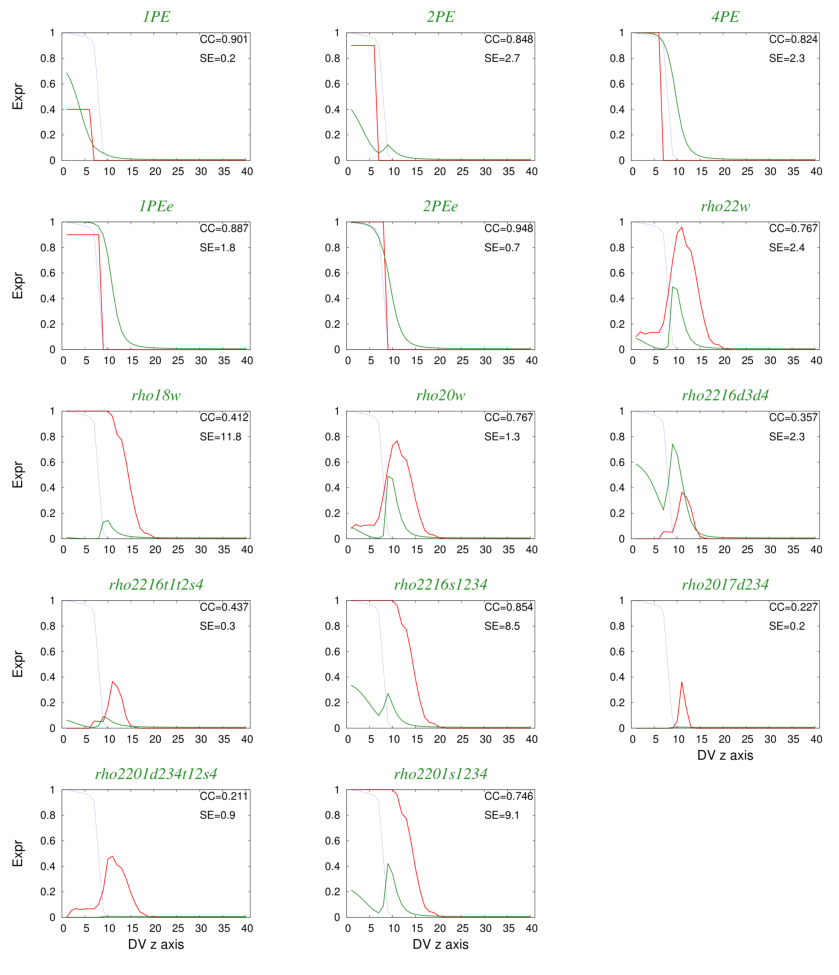
\includegraphics[width=1\textwidth]{DIb.pdf}\\
  \caption{the legend is in the upper right corner of the table, denoting the Observed profiles ( $E_t(z)$ ) as red, the model predictions as green along with the header above each figure denoting the CRM (gene target) in green, and the Dorsal morphogen profile  ( $E_{Dl}(z)$ ) as dotted blue curve. }\label{roughfit}
\end{figure}
  The correlation coefficient between the observed pattern and the predicted pattern is denoted as CC for each gene (which is at most 'one'), and also the squared error between the observed pattern and predicted pattern is denoted as SE for each gene (where each gene had 40 positions, z, along the DV axis (i.e. SE is at most 40).  The Snail profile is uniform from positions 0 to 8, where it is 'on' (at a value of 'one') and Snail is off from positions 9 to 40 along the axis, and the Twist gradient (profile) was replicated as the Dorsal gradient.
\newpage

%\begin{table}
%\begin{tabular}{|c|c|c|c|c|c|}
%\hline 
%\omega_{Dl,Tw}(d_1)&	\omega_{Dl,Tw}(d_2)&	\omega_{Dl,Sn}(d_1)&	\omega_{Dl,Sn}(d_2)&	w_{Dl}&	w_{Sn} \\
%\hline 
%5&	64&	.1&	.7&	7&	39 \\
%\hline
%1.872&	37& 25& 12& .05 & 687\\
%\caption{The errors were estimated as the square root of the diagonal of $(J^TJ)^{-1}$, where the parameters estimated are in first row of the table, and their values in the second row of the talbe, and their standard deviation in the third row.  The $\chi^2=41$, where we had 1200 data points (each position along the z axis for each gene).  The Hessian, had a high condition number ($10^4$) where the largest eignevalue was 1.4, and the two smallest eigenvalues were .0002 and .001, suggesting that $\chi^2$ surface was close to flat along these dimensions of parameter space (i.e. the null space).}
%\end{tabular} 
%\end{table}
%

\subsection{Redesigning the parameters to be fit}
 
 The results above suggest poor nonlinear regression model design or insufficient data, where the free parameters to be fit from \ref{freeparams} were based off Segal's thermodynamic model, which was similarly used by Xin in GEMSTAT and Fukhouri et.al.\cite{pmid20087339}.  In general, the more parameters we add to the nonlinear regression model will either decrease the $\chi^2$ statistic (albeit, the reduced chi-squared that accounts for the degrees of freedom may increase) or it will maintain the $\chi^2$ statistic at a particular value (\textit{i.e.} the statistic becomes insensitive to additional parameters); but the $\chi^2$ will not increase.  This assumes one's fitting algorithm is allowed to 'find' the point along the newly added parameter's line in parameter space that improves the fit or at least does not spoil the smaller parameter set's fit.  Spoiling a previous fit with a newly added parameter can be avoided, for example, by simply setting the new parameter to a value where the model is insensitive (and hence $\chi^2$ will not be disturbed).  For model's with extensive dependencies between parameters this may not be possible.  However, by inspection, the parameters of our nonlinear model can all be set to values such that they have no contribution to the $\chi^2$.  For example, all the parameters in our nonlinear model, when set to numerically one, have the effect of not influencing the form of the model, in a sense, this is the parameter free form of the model.  I will call these values of the parameters the default values (\textit{i.e.} the default values have the odd property that it appears we are not fitting the parameters at all; and, in another sense, one could imagine fitting all the parameters and all the parameters being fit to the default values. ).  While setting the values to be zero have the effect of 'knocking out' all binding sites of a factor (in the case of $\alpha$) or 'knocking out' pairs of interacting binding sites (in the case of $\omega$)). 
 
   Fitting subsets of the parameters in Eq.\ref{freeparams} (such as a parameter subset without our novel pairwise potential $\omega$) leads to good fits, by eye, of the data, such as RMSE's of .05.  However, upon implementation of a Hessian matrix using a two point finite difference, we found that the Hessian matrix was not full rank for the parameter set even without the pairwise interactions $\omega$, our novel form of the potential.  Without pairwise interactions, one still has six free parameters to fit for the CRM's responses to Dorsal Twist and Snail morphogens.  Based on expert knowledge of the DV network, certain choices of two of the parameters were selected to fit the data, which occasionally lead to a Hessian with a condition number of about 100 (the condition number is a numerical technique to determine if a matrix is singular\footnote{In a computer, in a numerical representation, a matrix is rarely actually singular, it just has some eigenvalues that are much smaller than the largest eigenvalue of the matrix.  The number of eigenvalues of Hessian is the number of parameters to be fit, and if some of these eigenvalues are close to zero, this suggest a zero determinant Hessian.}), while many of the choices of parameters lead to Hessians with condition numbers on the order of $10^4$.  Furthermore, the Hessian should be positive definite for a unique solution, while we found the eigenvalues were frequently mixed in sign (indicating saddle points) - of course the gradient (the derivative of the $\chi^2$ with respect to each parameter, a different object from the Jacobian) was zero (on the order of $10^-{10}$ for each component) at all of our estimates of the minima of the $\chi^2$ surface\footnote{These results lead to the implementation of the Levenberg Marquardt that has a number of GSL built in functions to help diagnose pathological nonlinear models (unlike the gradient descent and simplex implementations).  If Levenberg Marquardt revealed the same types of errors in our parameter estimates then we could be more confident that there was not an error in our implementation of the Hessian.  (i.e. a zero determinant Hessian, means our parameter error bars are infinite in extent - unless one decides to use a different method to estimate their error bars).}.
 
%  For example, the finite difference Hessian was found to be unstable for step sizes smaller than $10^{-^$ presumably due to 'catastrophic cancellation' (subtraction of two numbers with different number of significant figures).

In order to better estimate the errors of the parameters for our model we aimed to obtain a full column rank Hessian (regardless of whether the Hessian was positive definite).  We analysed the analytic derivative of our nonlinear model with respect to each parameter $\beta_i$, and checked if other parameters occur in the result (indicating dependencies between parameters).  If possible, parameters that do depend on one another were grouped to form just one parameter\cite{beck}.  Furthermore, certain regions of the Data space (such as certain positions in the embryo (like the dorsal ectoderm, where none of our genes are active) may be very insensitive to our parameters (causing small values of the Jacobian for these data points, however this does not appear to affect the Hessian of the $\chi^2$, since the analytic Hessian, $\mathcal H$ of the $\chi^2$ is exactly equal to $J^TJ+G$, where G is a matrix of second derivatives over the model\footnote{The analytic Hesssian in exact form is  $\mathcal H=\frac{\partial^2{\chi^2}}{\partial{\mathbf{\beta}}\partial{\mathbf{\beta}}} = J^TJ + \frac{\partial^2{f}}{\partial{\mathbf{\beta}}\partial{\mathbf{\beta}}} = J^TJ +G$, where G is matrix with second derivative elements of the nonlinear model f (the fractional occupancy of the BTA) over the model parameters (for example, see equation A.4c page 482 of Beck\cite{beck}).  In the case that G's Frobenius norm is nearly zero (the elements of G are nearly zero), then we have $\mathcal H=J^TJ$, which is why with certain data sets and experiments, it is possible to estimate the covariance matrix of parameters based on Jacobian alone.  $J^TJ$ for the case of one free parameter is just a dot product (i.e. the Jacobian is just a vector of size n x 1, where n is the number of data points), which will be insensitive to data points that were uninformative for parameter estimation (they're just adding a term zero to the dot product).  Hence, it seems reasonable that uninformative data (data where the model is insensitive, such as Dorsal ectoderm regions of the embryo, where none of our CRMs are active) will not cause harm to model fitting.}.  

%}.  Hence inverting the Hessian in the case that G is small (which it is for cases like the dorsal ectoderm data points, will require inverting $J^TJ$, but if there are many terms that are zero in the Jacobian (zero due to selecting data points where the model is insensitive to variations of the parameter), then $J^TJ$ will also be noninvertible (zero determinant).
\subsection{Analytic Jacobian }
A simple function is $f(z)=1/(1+\exp(-\beta z))$, where $\beta$ is a constant, where the domain and range of $z$ and $f$ are: $z \in [-\inf,\inf] \ \ f(z) \in [0,1]$.  Now if we imagine that $\beta$ was a free parameter, then we could ask how sensitive this function is to variations of $\beta$ as a function of particular positions along the domain of z.  Hence the derivative is:
\begin{equation}
 \frac{\partial{f(\beta,z)}}{\partial{\beta}}= \frac{\beta \exp{(-\beta z)}}{(1 + \exp{(-\beta z)})} \approx  \beta f(z,\beta) (1-f(z,\beta))
 \end{equation}
 The above equation, in a sense, is an analytic representation of the Jacobian matrix elements for the nonlinear model (e.g. BTA occupancy) as a function of data (all possible data, which is represented by the domain of z).  
 
 We do not need to analyze our more complicated BTA occupancy function to understand the behavior of the Jacobian matrix elements, rather we can simply use the above equation as a phenomenological parametrization of our model of CRM response to morphogen gradients (which are encoded in the spatial position $z$).  For example, imagine one wished to analyze phenomenologically the response of \textit{rhomboid} expression pattern just in the positions of the embryo of the neuroectoderm and the dorsal ectoderm (in our binning of the DV axis this would be equivalent to the z interval of [9,40], where the interval [1,8] contains the mesoderm, which we are uninterested in for the moment).  We can model the $rhomboid$ expression as a function of DV axis using the above equation, where we set $\beta$ to be negative since we must reflect the function about the 'switch' point where the gene is turned 'on (the point in space where $rho$ turns 'on' is at the neuroectoderm-ectoderm border).  \footnote{If we modeled the 'switch' point where the gene is turned 'off' (the point in space where $rho$ turns 'off' is at the mesoderm-neurectoderm border) we would not have to reflect our graph about the switch.}  We must also offset the position where the logistic function reaches $1/2$ max (which in the above equation is position $z=0$).  Hence we mush add a constant to the argument of the exponential $$f(z)=1/(1+\exp(\beta z -\beta_0 ))$$, where $beta_0 $ will define the $1/2$ max of the logistic function when $z\beta=\beta_0$.
 
The analytic Jacobian for these two parameters (as a function of data z):
\begin{equation}
\frac{\partial{ f}}{\partial{ \beta}} = \frac{-z\exp{(\beta z-\beta_0)}}{(1+\exp{(\beta z-\beta_0)})^2}=-z f(1-f)
\end{equation} \footnote{The logistic function when evaluated at a particular point $z'$ can be thought of as a Bernoulli Distribution, hence, the last expression is the variance of the Bernoulli distribution, where the function $f(x')$ at each point $x'$ happens to be the 'parameter' that describes a Bernoulli distribution (normally this parameter is denoted as 'p' for probability, where the mean of Bernoulli random variable is also p, and the variance of a Bernoulli random variable is p(1-p).  This is effectively how the BTA occupancy is described along the DV axis where $x'$ now denotes the position along the DV axis, and $\beta$ is a free parameter.}
\begin{equation}
\frac{\partial{f}}{\partial{ \beta_0}} = \frac{\exp{(\beta z - \beta_0)}}{(1+\exp{(\beta z-\beta_0)})^2}= f(1-f)
\end{equation}
\footnote{Do these two two equations span parameter space?  Recall previously we analyzed $\exp{(\beta_1 +\beta_2) z}$ for its behavior in the context of nonlinear regression.  Similarly for the logistic nonlinear model we would like to analyze $1/(\exp{(\beta_0 +\beta z)}$.  For example, and if one knows with certainty two independent data points $(y_1, x_1), (y_2,x_2)$, then we can transform to a simple linear model for the above equation, where one arrives at the following system of equations $\begin{pmatrix}  1&x_1\\ 1 & x_2\\ \end{pmatrix} \begin{pmatrix} \beta_0\\ \beta \\ \end{pmatrix} = \begin{pmatrix} \ln{\frac{y_1}{1-y_1}}\\ \ln{\frac{y_2}{1-y_2}} \\ \end{pmatrix} $.  Does this span the $\beta,\beta_0$ plane (the parameter vector space)?  The determinant of the design matrix is $x_2-x_1$, which suggest as long as the experimental design was such that the data points $x_1$ and $x_2$ are not too close together we could actually 'fit' $\beta_0$ and $\beta$.  However, one must be careful here, since data collected in regions of very large or very small $x_1$ and $x_2$, will cause the original response $y$ to become close 'one' or 'zero' causing the logarithm's value to be very large, possibly causing numerical issues.  This can be seen by symbolically solving for the eigenvalues of the design matrix, where we must solve for the roots of $(1-\lambda)(x_2-\lambda)-x_1=\det(X-\lambda I)=0$), where X is design matrix, and $\lambda$ is the eigenvalues of the design matrix.  This yields the quadratic $\lambda^2 +x_2\lambda+x_2-x_1$.  If $\lambda$ is zero (which means we would have a singular design matrix) we see that indeed $x_2=x_1$, which makes sense, we can't expect repeated measurements of the same position in space to tell us anything about the global behavior of the sigmoid (as defined by the $\beta$ parameters).  Solving the for the roots of the polynomial using the quadratic formula we have:
\begin{equation}
\lambda=-\frac{x_2 \pm \sqrt{x_2^2-4x_1}}{2},
\end{equation}
here we know constraints on the data due to the embryo size, where the DV portion of the embryo constrains $[x_1,x_2]$ to reside in the interval $[0,40]$, since there are only 40 cells along that axis.  Given the constraint on embryo size it seems we can at least say $\sqrt{4x_1}<x_2$.}

Now we can see some simple relations. First of all $J^TJ$ =0 if one only collected data in the dorsal ectoderm region of the embryo (where the logistic is nearly '1', meaning we can not invert that matrix (so J is not full column rank).  Similarly, if one just has Boolean data for the expression pattern of $rho$ along the z axis, say 00000001111111100000000=$\bm{E}_rho$, the only possible point where J is nonzero is at the borders  where the gene switches from off to on or vice versa.  Now imagine for an NEE gene that we have an expression pattern over space like 0000000101010100000000 where the switching behavior (10101010) is in the neurectoderm region of the embryo, while the other two regions are the mesoderm and ectoderm.  Using a mathematical metaphor, it is as if one has $J^TJ_{meso} + J^TJ_{neuro} + J^TJ_{ecto} =J^TJ = J^TJ_{neuro}$, since the regions in data space of $meso, \ ecto$ are insensitive to parameter variations, hence these regions in data space (the row space of $J$), act as labels to the null space of $J^TJ$ that is a subspace of parameter space (the column space of $J$). 



%, though, since the actual matrix expansion of the above form is in the form of a set of rank one eigenvectors of the matrix $J^TJ$ (spectral theorem)\footnote{If one has an underdetermined system, then $J^TJ$ will be singular, and hence will have a set of degenerate eignenvalues of zero; which correspond to a set of eigenvectors, these eigenvectors span the null space of the symmetrized matrix $J^TJ$,  I can \emph{choose} them to be orthogonal (always possible for symmetric matrices).  These eigenvectors are in the parameters vector space, while the labels $meso$ and $ecto$ are in the data vector space.  I suspect that it is these regions in the embryo's axis of measurement that I suspect are insensitive to parameter variations (and hence in some sense, could be used as labels for the matrix $J^TJ$).}.

\subsection*{Analysis of binding energy effects on occupancy}
For one binding site, we can compute the average occupancy, it is just the probability of the bound configuration $P(c=1)$ where $c=1$ is the configuration vector in the bound state (c takes on only two values 1 or 0 ).
\begin{equation}
\frac{\partial{P(c)}}{\partial{E(S)}} =  P(c)(1-P(c))
\end{equation}
This function's maximum is .25, which occurs at $P(c)=.5$.  Hence the greatest effect of energy on the occupancy of one site is at half max occupancy. 
% Furthermore, we can estimate the binding process as poison for small $P(c)$, in which case $P(c)(1-P(c))\approx P(c)$.  Hence, for low occupancy, the error in the occupancy is about $\sigma_{P(c)}=P(c)$, therefore $\partial{E(S)} = \sigma_{E(S)} = \frac{\sigma_{P(C)}}{P(C)}=1$. 
Assuming the differentials are standard deviations we have:
\begin{equation}
 \sigma_{P(C)}=|P(c)(1-P(c))| \sigma_{E(S)}.
  \end{equation}  
% Solving for $\sigma_{E(S)$ we have:
% \begin{equation}
%  \sigma_{E(S)= \frac{\sigma_{P(c)}}{|P(c)(1-P(c))|},
% \end{equation}
% which for small $P(c)$ the we have  $\sigma_{E(S)= \frac{1}{\sqrt{P(c)}}$.
%\textit{What is approximately the minimum energy that can influence the configuration vector?}     

% If one places constraints on the range that the free parameters are allowed to fit, we can put a bound on the maximum energy of a binding site that can cause a differential effect on our model of a specified size.  For example, we may be uninterested in effect sizes as small as $|df|=|.01|$, which means the fractional occupancy of the BTA has changed by .01.  For a module of just one site, what is the highest possible energy that can cause an effect size of this magnitude?
%
%We simply need to calculate $df/dE$ analytically, and then solve for dE, setting df equal to .01.  It is helpful to analyze the effect of  energy sizes on the occupancy of morphogens (i.e.$ d<n>/dE$).  Here we will just analyze one binding site (therefore the expected occupancy of the binding site is equal to the probability of the site being bound $<n>=P(c_b)$, where $c_b$ is the bound configuration.
%
%\begin{equation}
%\frac{\partial{n}}{\partial{E(S)}} = E(S) <n>(1-<n>)
%\end{equation}
%  
%Hence the change in occupancy when there is a mutation in the site that increase the energy by $E(S)$ will have the effect $\partial{E(S)}$ and the :
%  \begin{equation}
%\partial{<n>}= (\partial{E})^2 <n>(1-<n>)=
%\end{equation}
%The variance of a boolean variable $<n>(1-<n>)$ is maximal at $<n>=1/2$, hence at half max occupancy the occupancy is most sensitive to perturbations of the energy. We would like to know what is the energy required to have an effect as small as $|d<n>|=|.01|$, which means the fractional occupancy of the morphogen has changed by .01.  In general we have:
%\begin{equation}
%\partial{E}=\sqrt{\frac{|d<n>|}{<n>(1-<n>)}}.
%\end{equation}
%Hence, for the case of interest we need to plot the function:
%\begin{equation}\label{difE}
%\partial{E}=\sqrt{ \frac{.01}{<n>(1-<n>)} },
%\end{equation}
%which is shown in figure \ref{diffE}:
%\begin{figure}
%  \includegraphics[width=1\textwidth]{diffE_3ener.eps}\\
%  \caption{Three different binding energy levels are analyzed, 1 (blue), 5 (red), and 10 (green).  At each energy level $\partial E=dE$ is calcualted from Equaton \ref{difE} to determine the amount of energy required to obtain a 0.1 increase in the occupancy of binding sites at that energy level. }\label{diffE}
%\end{figure}

%An energy of 9 is a Boltzmann factor of $\exp{(-9)}=.0001$, and energy of 4 is a factor of $\exp{(-4)}=.02$.  In our model the weight of a CRM with a single site in the bound configuration ($c_b$), has the following Boltzmann factor, $W(c_b)=q_i=K(S)[tf(i)]=K_0\exp{-E(S)}\frac{E_{tf}(k)}{E_{tf}(max)} = \exp{-E(S)}E_{tf}(k) \alpha_{tf}$.  We only use two significant figures for the expression data, hence the minimum value of $E_{tf}$ (excluding zero) is 0.01.  $\alpha_{tf}$ is the a free parameter to be fit bounded between $[1,100]$, hence the minimum value of $\alpha$ is 1.  Hence, the configuration weight with the smallest possible parameter and concentration case for an energy of 9 has a configuration weight for the bound case $W(c_b)= .01*.02=.0002$.  For modules with two identical binding sites of this energy, when all the sites are bound we would have a configuration weight of $(.0002)^2$ .  While the configuration weight with largest possible parameter ($\alpha_{max}=100$) and concentration ($E_{tf}(max)=1$) results in $W(c_b)=\alpha_{max}*E_{tf}(max)\exp{(-E=9)}= 100*1*.02=2$.  For modules with two identical binding sites of this energy, when all the sites are bound, then we would have a configuration weight of $(2)^2$.  Hence, in the case that $\alpha=100$ and $E_{tf}=1$ for a binding energy of 4, we see a binding site with energy 4 is actually at half max occupancy $<n>=1/2$; and that if the CRM had two binding sites of this energy, then the module reaches one full unit of occupancy of the transcription factor $<n>=1$ under peak concentrations and peak values of $\alpha$ (which is like a factor that has a large $K_0$).  We won't go through in detail the case of 9, but we do want to see that under peak conditions we would have $W(c,b)=\alpha_{max}*E_{tf}(max)\exp{(-E=9)}=100*1*.0001=.01$.  This $1\%$ the size of the weight for the unbound case $W(c_u)=1$, this means $<n> \approx .01$.  
%
%The effect of the occupancy of the morphogen on the BTA is based on our model: ($f_{BTA} = logit(w_0 + \sum_{tf } \ w_{tf} < n_{tf} > )$, where we have written our model in terms of the famous logit function which is the 'canonical link' to the odds of the $f_{BTA}$.  Hence, the log odds is:
%\begin{equation}
%   \log{\frac{f}{1-f}}= w_0 + \sum_{tf } \ w_{tf} < n_{tf} > 
%   \end{equation}   
%now if we take the log \emph{odds ratio}, where we assume $df= f_f - f_i=0.01$ is due to an increment in the energy $dE(S)$ (a yet to be determined increment in energy, which hereafter will be called $\Delta \epsilon$), where $f_i$ is the initial occupancy of the BTA, and $f_f$ is the final occupancy of the BTA, we then have:
%
%\begin{equation}
% \log{\frac{f_i}{1-f_i} \frac{1-f_f}{f_f}}=  w_0 - \sum_{tf} \ w_{tf} < n_{tf} >_i  - (w_0 - \sum_{tf } \ w_{tf} < n_{tf} >_f ).
%\end{equation}
%Now we now the log odds is zero when the occupancy of the BTA is half max.  Hence we have:
%\begin{equation}
% \log{\frac{1-f_f}{f_f}}=\log{\frac{.4}{.6}}=  \sum_{tf } \ w_{tf} < n_{tf} >_f   - \sum_{tf } \ w_{tf} < n_{tf} >_i 
%\end{equation}
%Now, assuming the CRM has just one binding site we for a transcription factor $tf$ we have:
%\begin{equation}
% \log{\frac{1-f_f}{f_f}}=\log{\frac{.4}{.6}}= \ w_{tf}( < n_{tf} >_f  -  < n_{tf} >_i ),
%\end{equation}
%where we can treat the energy decrement $\Delta \epsilon$ from the initial binding site to the new binding site as a perturbation factor in the canonical partition function, q, we then have:
%\begin{equation}
%  < n_{tf} >_f  -  < n_{tf} >_i = \frac{1}{1+q\exp{(-\Delta \epsilon)}} - \frac{1}{1+q}
%\end{equation}
%creating a common denominator and using the symbol $y=\exp{(-\Delta \epsilon)}$ we have:
%\begin{eqnarray*}
%\frac{1}{1+qy} - \frac{1}{1+q} &=& \frac{ q(1+y)}{(1+qy)(1+q)}\\
%&=& x,
%\end{eqnarray*}
%
%here x is the value of the log odds ratio, which we know.  Now after some algebra we arrive at:
%\begin{equation}
%\Delta \epsilon = -\ln{ \frac{  x (1+q)/q -1  }{ x(1+q) + 1}  }
%\end{equation}
%The value of the log odds ratio was 0.4, hence, an increment of $20\%$ of the occupancy of the BTA, in this case, is from a change in the binding site energy (due to a new binding site sequence) of:
% \begin{eqnarray*}
%\Delta \epsilon &=& -\ln{ \frac{ .4 (1+\alpha_{max}E_{tf}(max)\exp{-E(S)})/(\alpha_{max}E_{tf}(max)\exp{-E(S)}) -1  }{ .4(1+\alpha_{max}E_{tf}(max)\exp{-E(S)}) + 1}  }\\
%&=&-\ln{ \frac{ .4 (1+100\exp{-E(S)})/(100\exp{-E(S)}) -1  }{ .4(1+100\exp{-E(S)}) + 1}  }\\
%&=& 9.2
%\end{eqnarray*}
%Here we have assumed the initial binding site has $E(S)=0$, the ground state, furthermore we assumed that $w_{Dl,BTA}$ was 1.   

\subsection*{Balanced Data sets of mesoderm and neurectoder enhancers, Experiment 2}
The parameters of the thermodynamic model are all contingent on the free parameters that correspond to Snail (such as it $\alpha$ for its protein-DNA interaction, and its quenching strength, and its $w_{SN}$ for Snail's strength of repressing BTA binding).  Hence, to disentangle the cooperativity of Twist and Dorsal (if it exist) from the other free parameters, an experiment was conducted with no Snail protein (no Snail in the network).  Hence, the MPA simply annotates for Twist and Dorsal (where again the MPA was not 'fit' rather default parameters were set for annotation).  All NEE modules are known to be repressed by Snail in the mesoderm.  However, the cooperativity of Dorsal and Twist is known to be important when there are limiting concentrations of Dorsal in the neuroectoderm (where Snail protein does not exist).  Furthermore, the modules that are not NEE's (such as mesoderm targets of Dorsal), are know to have no Snail binding sites in their module (at least this will be hypothesis).  Here we used four CRMs to fit two parameter, the Dorsal binding strength and Dorsal-Twist cooperativity.  We found a $\chi^2=8.9$ for 80 data points\footnote{The goodness of fit can be tested here, with 78 degrees of freedom, we can assume our fit is a deviate from the $\chi^2$ distribution.  If the value of our squared error is a reasonable deviate from the $\chi^2$ distribution then we can accept the fit.  I computed the p-value as nearly one, suggesting the fit is good (the cdf of our the $\chi^2$ distribution to the value we found was $10^{-28}$. }.    We removed the constraint on the parameter ranges, and set $w_0= 5$,  $w_{Dl}=-5$, $w_{Tw}=0$.  We set $w_{Dl}=5$ because we wanted one unit of Dorsal occupancy to correspond to half max BTA occupancy (which means the target gene is at half max).  We set $\alpha_{Tw}=1$, the default value.  We found $\alpha_{Dl}=0.3 +/- 0.03$, and $\omega_{Dl,Tw}=3980 +/- 982$, where the standard deviations were estimated from the square root of the corresponding parameter's diagonal element of $(J^TJ)^{-1}$.  The   

These results are as expected from the modules shown.  For example, the construct $6xdl$ was a Szymanski construct that was shown that even with 6 Dorsal binding sites, the CRM does not respond to Dorsal in the neuroectoderm (see profile in Figure).  Hence, if these were zero energy Dorsal sites, then we know for what was defined as the minimum value of $\alpha_{min}=1$ that Dorsal occupancy would reach half max at the position z and a concentration $E_{Dl}(z)$, hence we have: $E_{Dl}(z)/(1+E_{Dl}(z))=<n_{Dl}>= 1/2$, hence $E_{Dl}(z)= 1$.  However, the CRM $6xdl$ had 6 Dorsal binding sites, hence one unit of occupancy could be reach at 1/6 this concentration (since the sites are all independent, by assumption).

Another construct that was used was the double knock out of Twist sites by Ip, which reported catastrophic loss of expression in the neuroectoderm, the construct labelled $rho2216t1t2s4a$.  Hence the Ip construct along with the $6xdlPLZ$ acted as a control group.  The treatment group (in a sense) were two constructs that are known to have Twist sites the $rho$ CRM (from $mel$ specie), and the $vn$ CRM (from $vir$ specie).
 
The Snail protein was not used in this model, , and the Twist gradient (profile) was replicated as the Dorsal gradient.  The $6xtwPLZ$ was also left in the training set, but this has negligible effect (due to model assumptions (i.e. default parameter values of Twist), and the reported expression profile by Szymanski for a this construct was roughly zero (i.e. Twist binding sites alone are not sufficient)).
\begin{figure}
  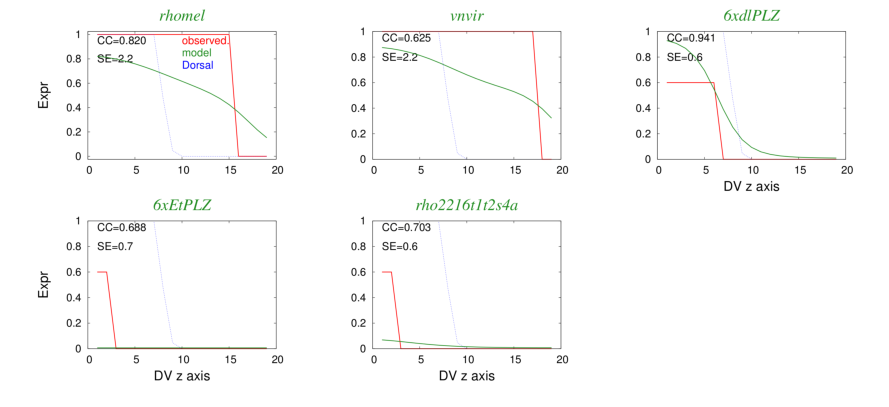
\includegraphics[width=1\textwidth]{DInosnail.pdf}\\
  \caption{the legend is in the upper right corner of the table, denoting the Observed profiles ( $E_t(z)$ ) as red, the model predictions as green along with the header above each figure denoting the CRM (gene target) in green, and the Dorsal morphogen profile  ( $E_{Dl}(z)$ ) as dotted blue curve.  The correlation coefficient between the observed pattern and the predicted pattern is denoted as CC for each gene (which is at most 'one'), and also the squared error between the observed pattern and predicted pattern is denoted as SE for each gene.  Each gene had 20 positions, z, along the DV axis, which as always (in DV literature), is plotted such that ventral is at the zero position.  }\label{roughfit}
\end{figure}


\begin{figure}
  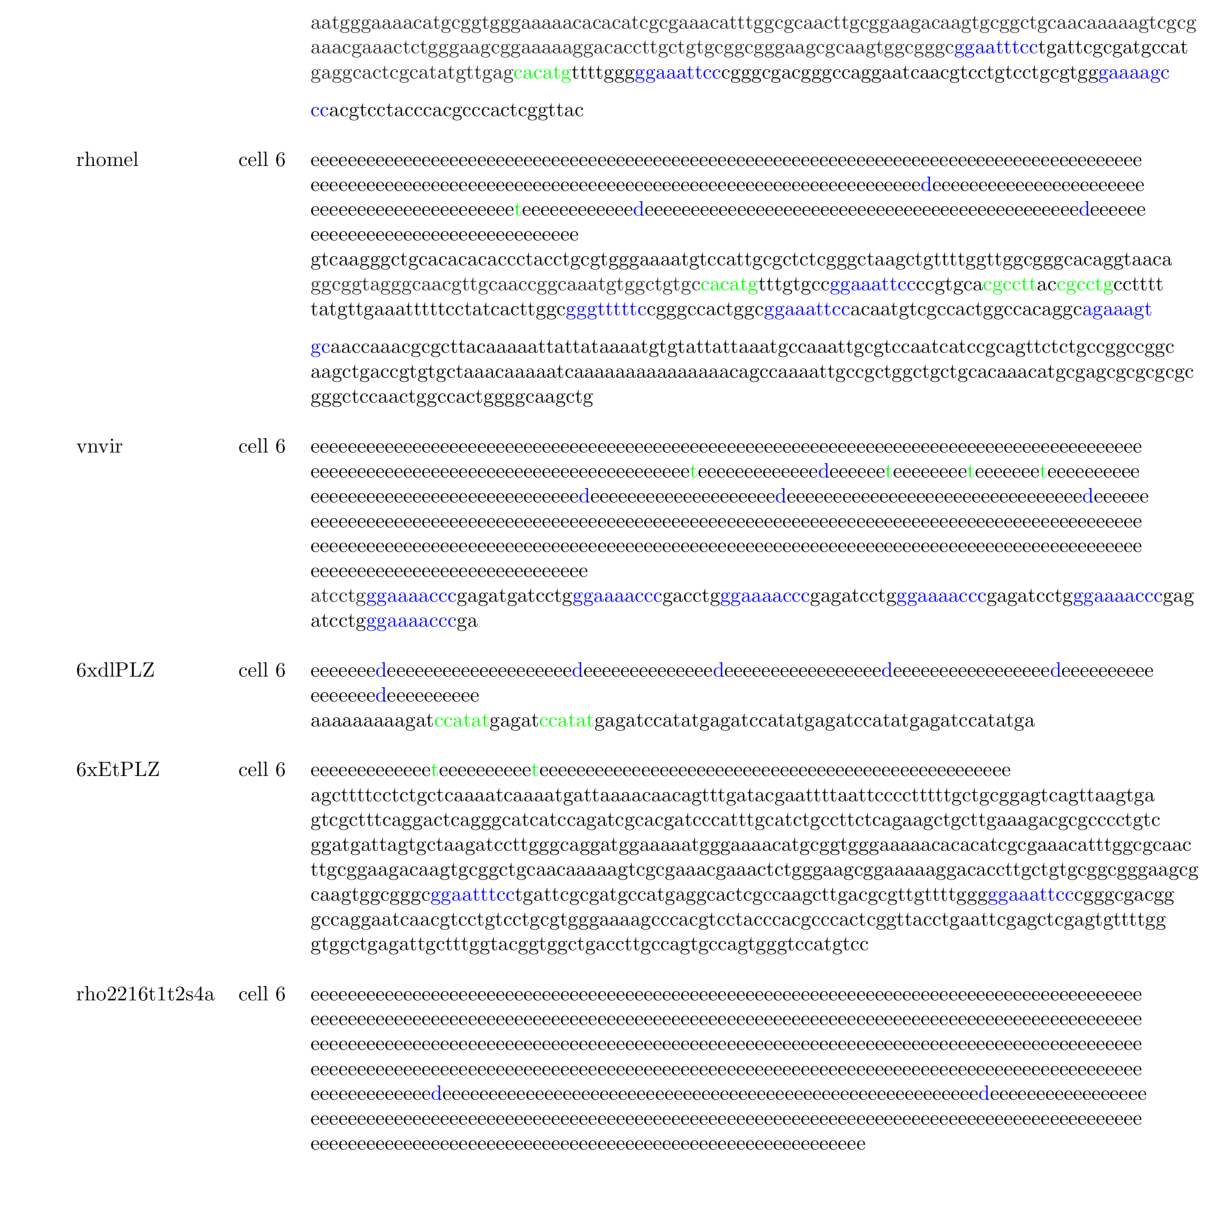
\includegraphics[width=1\textwidth]{annNosnail.pdf}\\
  \caption{The CRMs and predicting binding sites from MPA for default parameters on all proteins.  Dorsal annotated blue, Twist green. The column d+ denotes added noise to Dorsal concentration profile (which was zero in this case, hence d+ should not be there).  A bug in the printing code caused one of the $vnvir$ sites to not appear in the CRM sequence highlighting. }\label{roughfit}
\end{figure}
%Hence we could simply not model the mesoderm, and contrast NEE's that have variation in their patterns from the dorsal ectoderm to the ventral-most region of the Neuroectodem (the mesoder-neuroectoderm border).




\subsection{Robustness analysis, Experiment 3 }
We increased the Dorsal expression by .15 in each position along the DV axis to see if the annotated binding sites were the same when using the annotation model MPA.  The data set was four NEE modules $rhomel, rhovir, vnmel, vnvir$.


The Twist gene's free parameters were all set to 'one' for $\alpha$, and $\omega_{Tw,Dl}$ was set to 'one' for all bins except $B=[0,20]bp$, and $w_{Tw}$ parameter was set to zero.  Furthermore, the Twist's morphogen concentration gradient $\bm{E_{Tw}}$ was set equal to Dorsal's gradient to assure their differential gradients were not influencing the result.  Snail's quenching was set for $w_{Sn,Dl}$ for only one bin $B=[0,50]bp$ (quenching means $\omega$ is in the range [0,1], while cooperativity means $\omega$ is in the range [1,100].  Hence, we only allowed the Dorsal and Snail parameters to be tuned by the fitting routine.
 
The results of annotation with the wild-type Dorsal expression (no perturbation of the profile) are in figure\ref{annb}.  The results of the perturbed Drosal profile are in figure \ref{annc}.  The annotations are the identical.  This possibly is an artifact of the way the Dorsal profile was perturbed (by simply adding .15 to each cell).  Due to the sigmodal nature of the Dorsal profile this has little effect.  A better designed experiment would shift the half max of the Dorsal profile by a fixed number of positions along the z axis.


%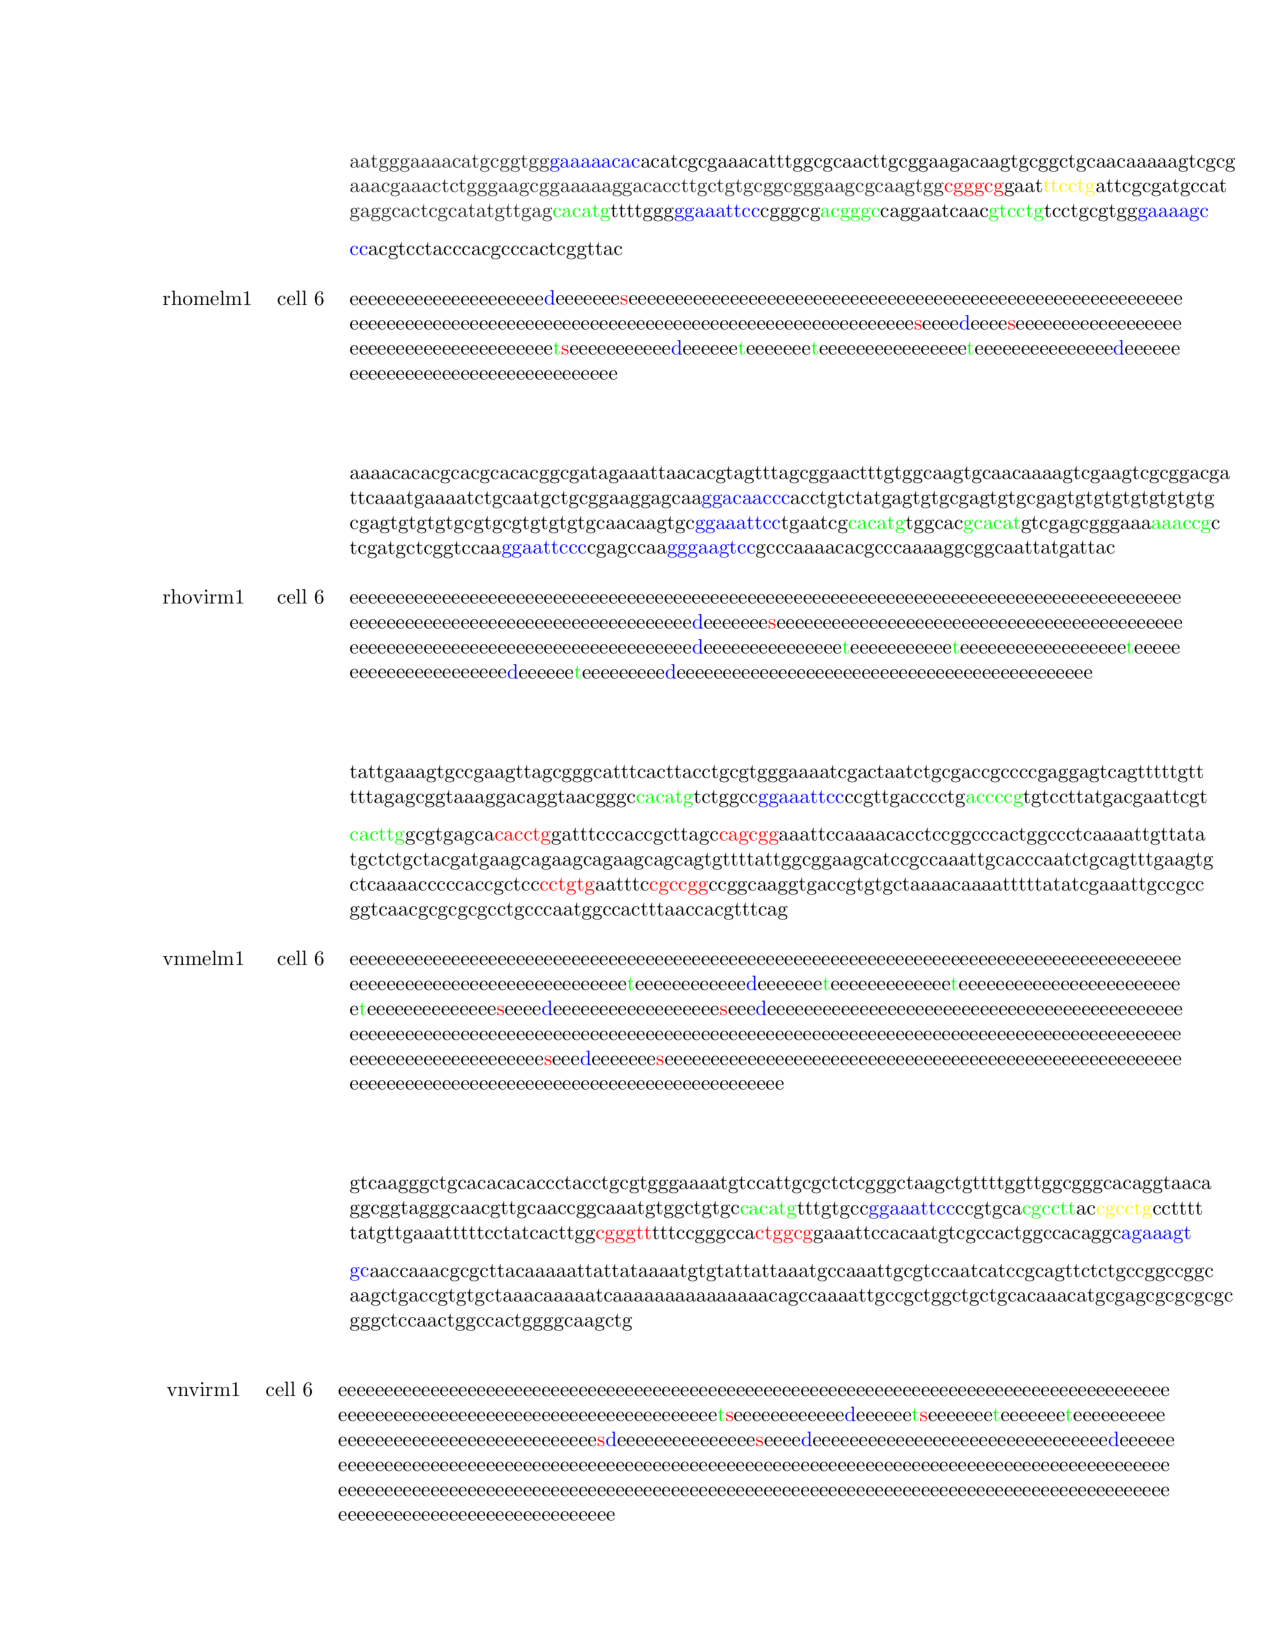
\includepdf[pages=-]{annb.pdf}
\begin{figure}
  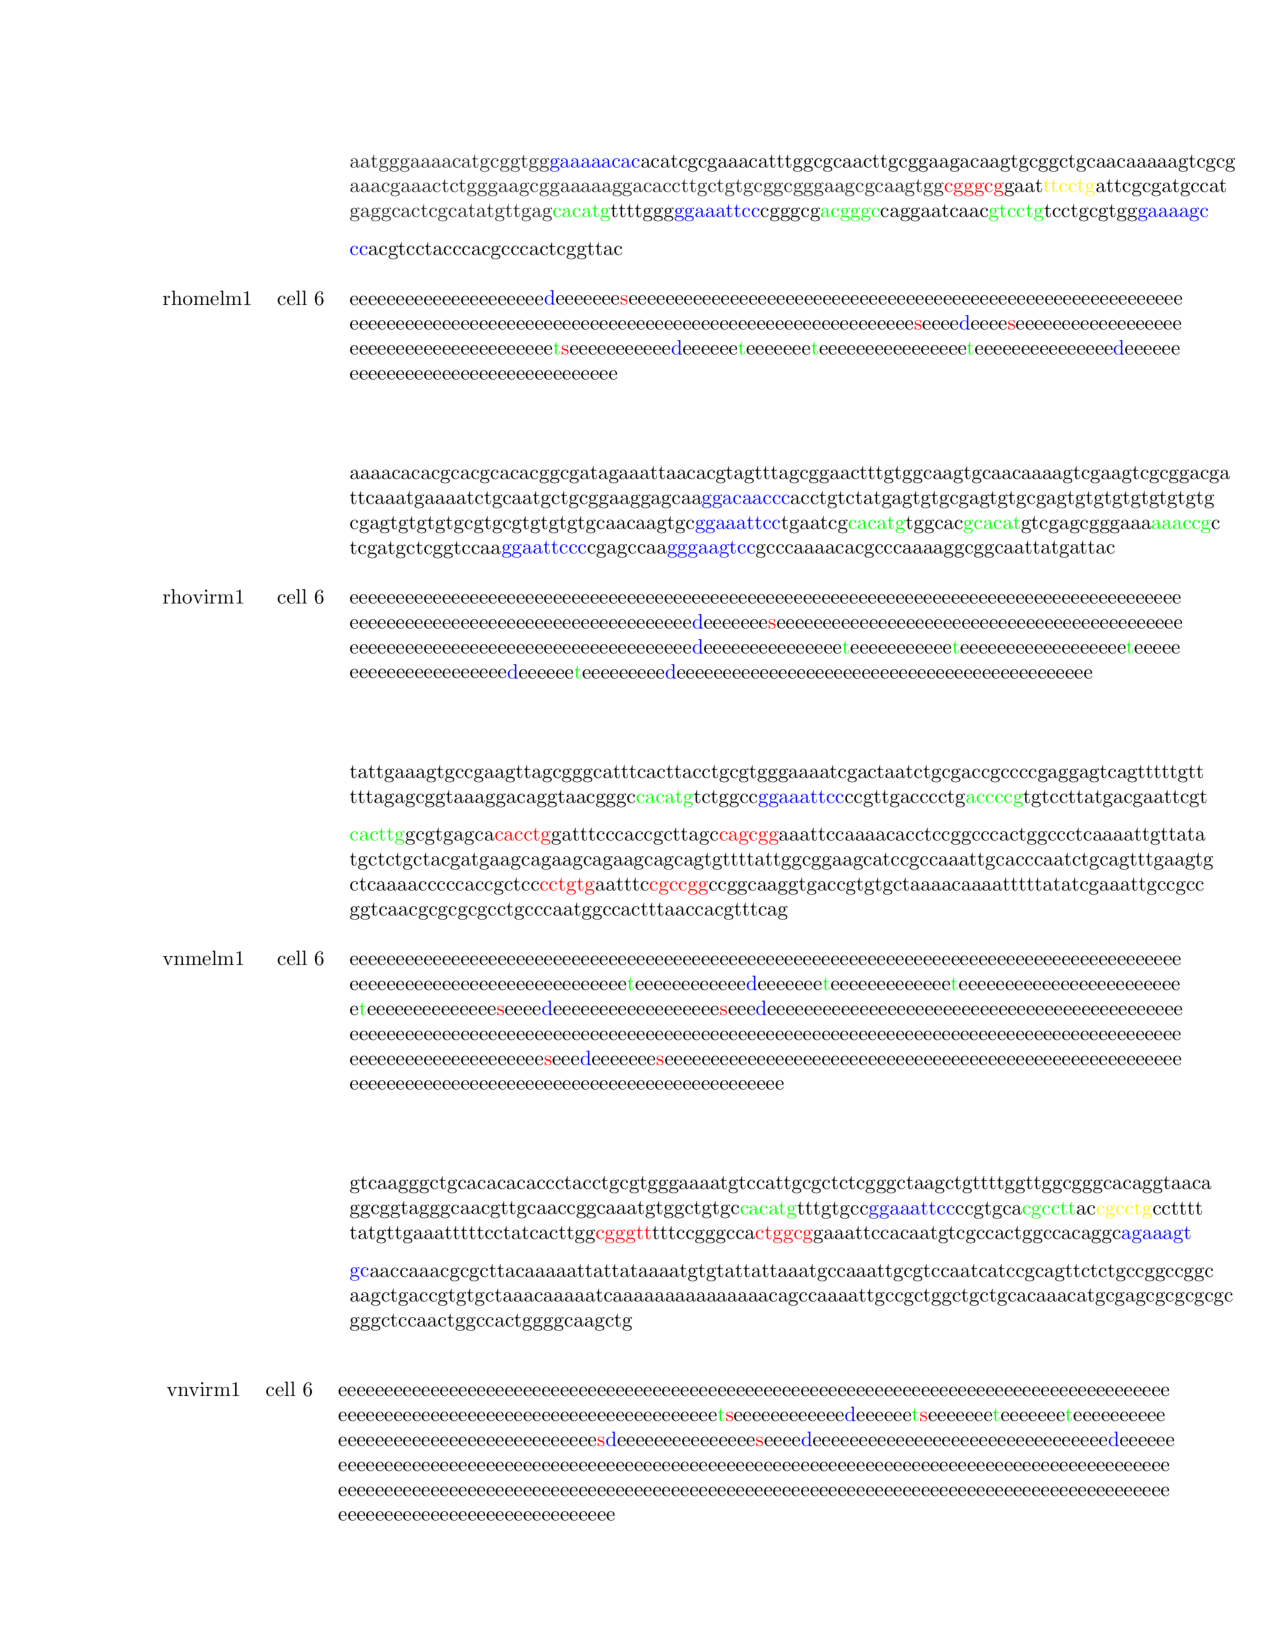
\includegraphics[height=1\textwidth]{annb}\\
  \caption{Here the target gene is denoted in the left column, and the cell along the DV axis is denoted in the second column.  Twist site's are annotated green, Dorsal blue, Snail red, and brown denotes overlaps.  The sites annotated at the mesoderm bottom border were used to annotate the sequence.  For example, the first gene is $\emph{rhomel}$, for \textit{rhomboid} in the species $melanogaster$. }\label{annb}
\end{figure}
%The expression profiles for the above CRMs are shown in following graphs, where the annotated binding sites were based on the gene's corresponding annotation from the mesoderm 'm1' condition.  In addition to showing the correlation coefficient (CC) between model and observations, and the squared error between model and observations (SE), we show the absolute error (AE), which is the absolute value of the difference between the model predictions and the observed pattern. 

%\includepdf[pages=-]{DI.pdf}

%\begin{figure}
%  \includegraphics[height=.8\textwidth]{DI.pdf}\\
%  \caption{the legend is in the upper right corner of the table, denoting the Observed profiles ( $E_t(z)$ ) as red, the model predictions as green along with the header above each figure denoting the CRM (gene target) in green, and the Dorsal morphogen profile  ( $E_{Dl}(z)$ ) as dotted blue curve.  The correlation coefficient between the observed pattern and the predicted pattern is denoted as CC for each gene, and also the squared error between the observed pattern and predicted pattern is denoted as SE for each gene (where each gene had 40 positions, z, along the DV axis.  The Snail profile is uniform from positions 0 to 8, where it is 'on' (at a value of 'one') and Snail is off from positions 9 to 20 along the axis, and the Twist gradient (profile) was replicated as the Dorsal gradient. }\label{roughfit2}
%\end{figure}
\begin{figure}
  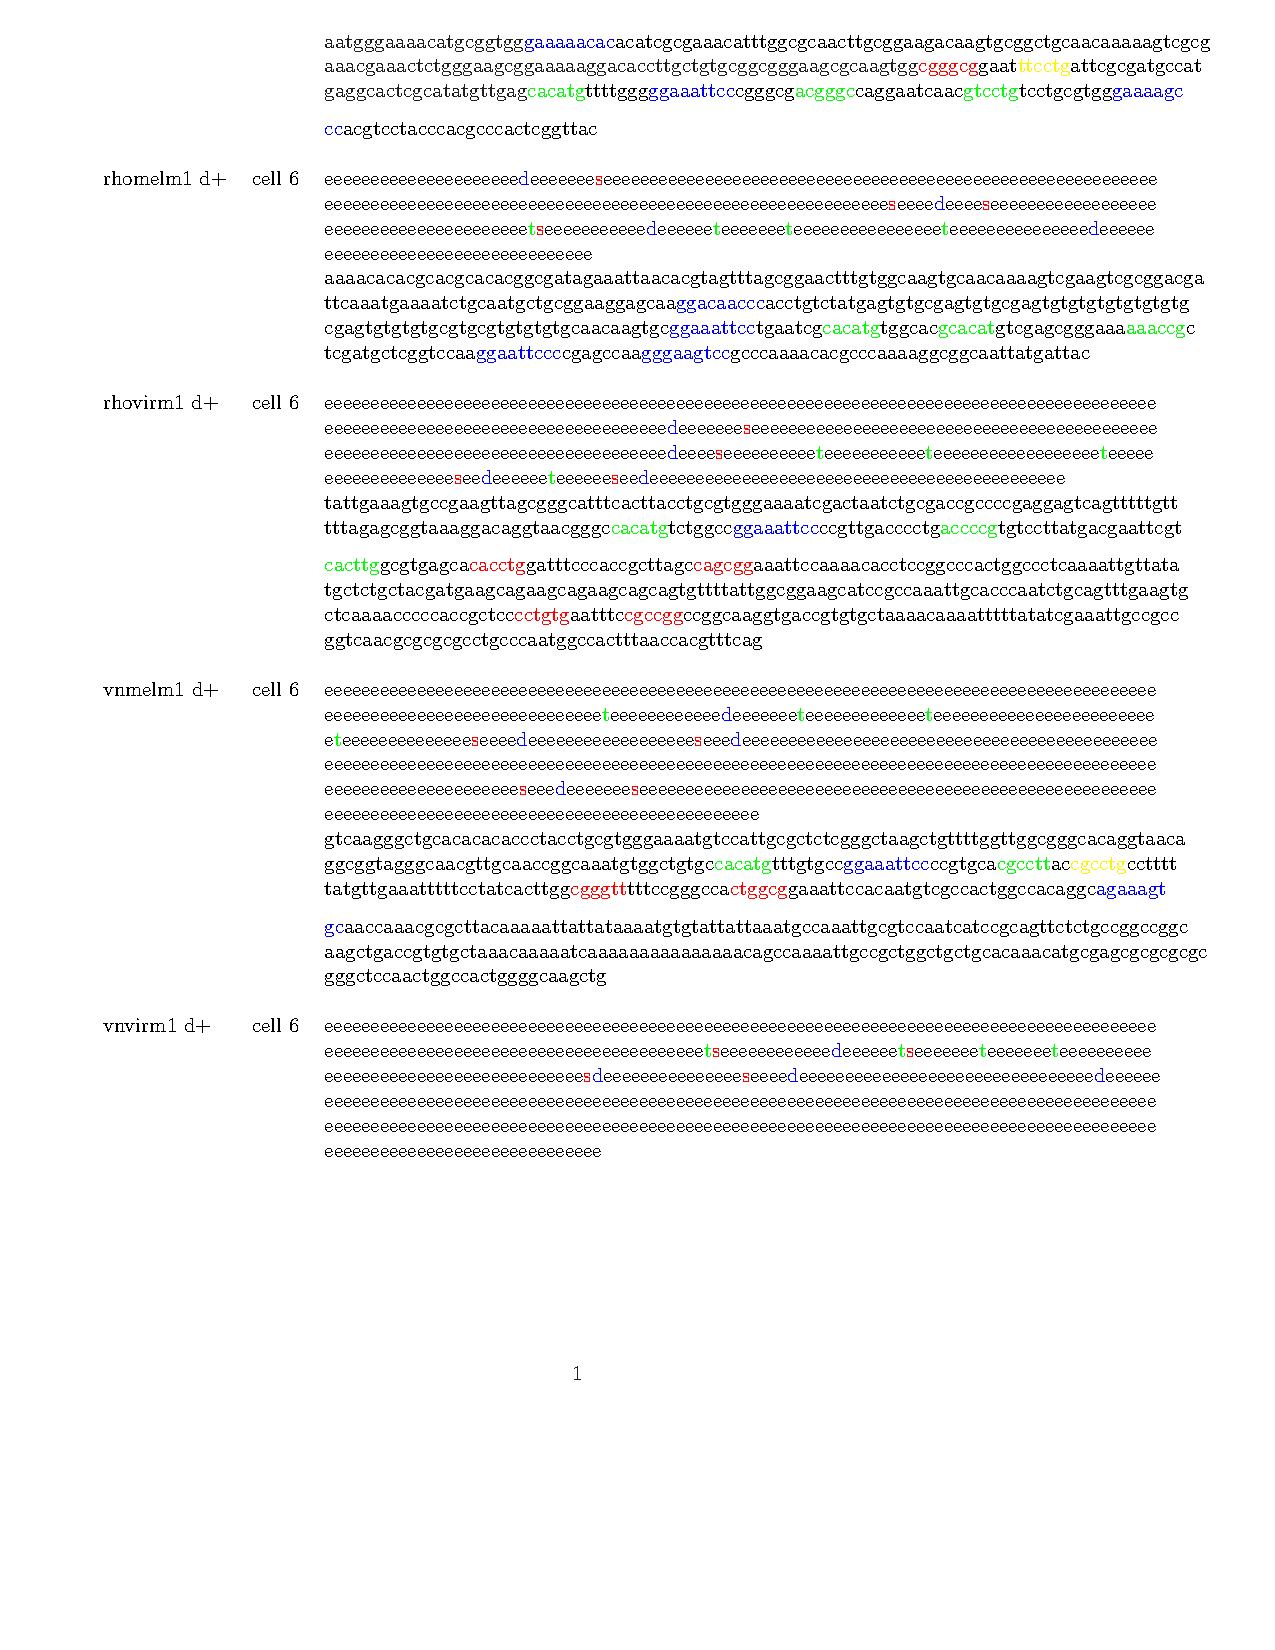
\includegraphics[height=1\textwidth]{annc}\\
  \caption{Here the target gene is denoted in the left column, where, where the second column contains d+ to denote an in increase (+) in the Dorsal (d) gradient along the DV axis, and the cell along the DV axis used for extracting concentrations for the annotation model MAP is denoted in the third column.  Twist site's are annotated green, Dorsal blue, Snail red, and brown denotes overlaps. }\label{annc}
\end{figure}

\section{Discussion and Background on Robustness}
\subsection{Morphogen Gradients and Developmental Robustness}

Given a morphogen distribution over one spatial dimension, one can determine how sensitive the thresholds of the target genes are to perturbations of the morphogen distribution.  This is discussed in Alon's text in chapter 8 "Robust Patterning in Development" \cite{designp}.  Here we will reproduce Alon's derivations for producing a morphogen profile ( distribution ) and his analysis of whether this profile is robust, but we will do so in the context of the morphogen Bicoid and its robustness probe Hunchback, where similar analysis was done by Gregor and Houchmandzadeh \cite{pmid17632062}\cite{pmid11845210}.  Our analysis starts with a transport equation for the morphogen.
\begin{equation}\label{}
    \frac{\partial M}{\partial t} =  D \frac{\partial^2 M }{\partial x^2} - F(M)
\end{equation}
Here $F(M)$ is a function of the morphogen concentration and represents the degradation of the morphogen.  Notably missing from the equation is the production rate of the morphogen, as assumed from Gregor and in Alon's text the morphogen is assumed to be in steady state\cite{designp}.  Hence the time derivative is zero, and one can determine, or declare, the morphogen concentration by the boundary conditions:
$
    M(x = 0) = M_0 $ and $  M(x=\infty) = 0
$
 It is important to conceptually see what these conditions mean, since thermodynamic equilibrium in diffusion processes would lead to a morphogen distribution that is uniform over space, which we're about to see is not the case for our problem because a uniform profile occurs only if the system does not have sources and sinks.  Here we're assuming some source, a constant source such as ribosomes translating Bc mRNA at position x=0, and we are assuming a sink by the proteasome degradation of the Bc protein at $x=\infty$. \footnote[1]{ the idea that Bc mRNA is localized at x=0 was recently shown false, it was shown that Bc mRNA is also diffusing and closely follows the Bc protein profile, but for our discussion we'll assume that Bc is translated into protein at x=0 and then diffuses, and all of this is captured by our boundary condition.}
The Diffusion constant D determines the \textbf{absolute} length scale of the problem, which creates a problem for patterning mechanisms if the embryos have large variations in their size, since an intricate \textit{scaling} mechanism would be required, as diffusion is based on absolute length scales, this is discussed by Gregor and by Crocker \cite{pmid18328473}.  Assuming the variation of the embryos length is negligible we need to see how the scale of the problem is established. Alon's analysis starts with a linear degradation mechanism $F(M) =\alpha M $, where upon solving the PDE given the morphogen is in steady state, one arrives at:
\begin{equation}\label{ss}
    M(x) = M_0 e^{-\frac{x}{\lambda}}
\end{equation}

where $\lambda = \sqrt{\frac{D}{\alpha}}$, clearly when $x=\lambda$ the morphogen has reached a concentration of $\frac{M_0}{e}$, which is only about 33\% of its max, and after $2 \lambda$, the morphogen has reached a concentration of $\frac{M_0}{e^2}$ in general:
\begin{equation}\label{}
    x = \lambda, 2\lambda, .. n \lambda
\end{equation}
then
\begin{equation}\label{morpscale}
    M = \frac{M_0}{e},\frac{M_0}{e^2},..\frac{M_0}{e^n}
\end{equation}
 Using 'units' of $\lambda$ is not only useful for seeing how the morphogen decays as a function of absolute length, it is in fact the units the morphogen uses to create patterns, as when one anthropomorphizes the morphogen, they realize that the morphogen can not reproducible 'make' patterns on any scale other than $ \lambda $, where reproducible means comparing the patterns \textbf{between} embryos.


  \subsection{Fine patterns}
   Let's see if the morphogen 'can create' a fine pattern on the scale of $ 1 \mu m = $ when $ \lambda = 10 \mu m$. Now the morphogen creates the pattern by binding to the Hb promoter and stimulating Hb expression, so the Hb expression as a function of space is the 'pattern'.  This is denoted by figure \ref{shift}.  In drosophila the x axis (the Anterior Posterior axis, major axis of the elliposdal embryo) is about 500 $\mu m$ and each nucleus is separated by about 10 $ \mu m$, since the pattern here is referring to the expression of Hb as a function of nuclear position, we see that $ 1 \mu m$ doesn't even make sense, since the smallest unit of our problem is $10 \mu m$,  So let's fix our ill-posed question to the morphogen trying to make a pattern over  $ 10 \mu m $ where $ \lambda =100 \mu m $.  Now to determine if a pattern can be created all we need to know is if the Hb promoter can detect (distinguish) Bc concentrations that are separated by $ 10 \mu m $  (two neighboring nuclei).  Well the answer is simple, \textbf{yes}, if we use the Hill model \eqref{segcon2hb}, to represent Hb's detection mechanism, then clearly the promoter can detect \textbf{any} concentration of Bicoid, and clearly any desired pattern could be produced  (To determine the pattern one simply defines a Bicoid concentration as the start of the pattern (i.e. a 'threshold concentration', M(x)) and and then inverts the Hill equation to find the Bc concentration and position, which come from equation \eqref{ss}).
 \begin{equation}\label{segcon2hb}
    \frac{[Hb]}{[Hb_{max}]} = \frac{1}{1 + e^{ -(w_{0} +  \left< n_{Bc} \right> w_{Bc}})}
\end{equation}

 But, we want to explore this problem from the perspective of robustness, that is if the Bc concentration deviates from its ideal profile for whatever reason (e.g. the mother laid less functional bc mRNA because only one of her bc alleles is functional (heterozygote ), or a slight variant of mRNA are laid in the oocyte etc..) , then what would happen to our Hb profile.  In this sense, one may loosely say that we are interested in knowing if a nonrobust input can still be transformed into a robust output \footnote[2]{for thermodynamic modeling (fractional occupancy) this question is approximately answered by taking the derivative of the model $<N_{mRNA}>$ with respect to the input concentration that is varying, one will see that the effect is only at the border due to the form of the model}.

  A formal measure of this (robustness) is defined by Alon as the 'positional shift' that is by how many microns $\delta $ does our pattern shift.  To determine the function $\delta $ we need to perturb the production rate M (i.e. the boundary condition at x = 0) from $M$ to $M'$, then one can see $\delta $ from the graph in figure \ref{shift}.  When analyzing these equations, keep in mind that the Hb concentration is captured by the concentration of the morphogen [M], so M(x) and M(x') represent the same Hb concentration.
  \begin{equation}\label{inverse}
    d x = \frac{d x }{d M} dM
  \end{equation}

\begin{equation}\label{solvex}
    dx = \delta = x - x'
  \end{equation}
  inverting equation \eqref{ss} we can isolate the position, hence solving for x:
  \begin{equation}\label{}
   x = \lambda \log{\frac{M}{M(x)}}
  \end{equation}
  now if we change the boundary condition to M', and solve for x', which represent the new border position of Hb expression:
  \begin{equation}\label{}
  x' = \lambda \log{\frac{M'}{M(x')}}
  \end{equation}
  now we have the pieces to calculate $\delta$,
  \begin{equation}\label{}
     \delta = \lambda \log{\frac{M}{M(x)} }- \lambda \log{\frac{M'}{M(x')}}
  \end{equation}
  since M(x) = M(x'), we arrive at:
  \begin{equation}\label{}
  \delta =  \lambda\log{\frac{M'}{M}}
  \end{equation}

\begin{figure},
  % Requires \usepackage{graphicx}
  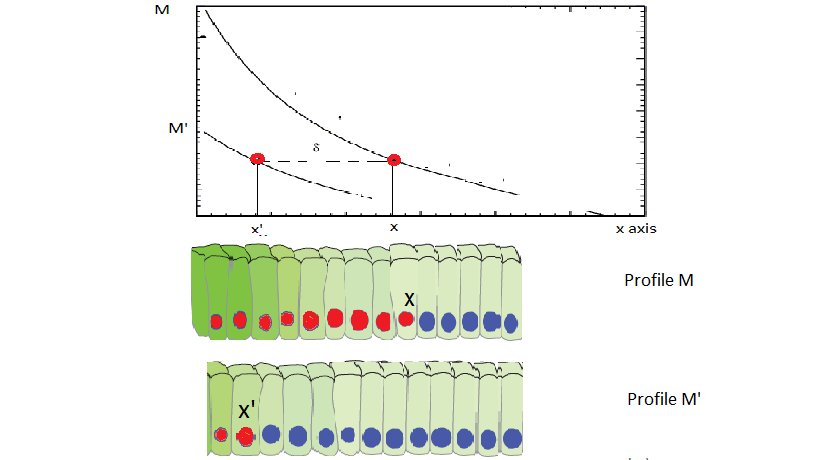
\includegraphics[width=1\textwidth]{sourcegraph}\\
  \caption{the green gradient represents the concentration of Bicoid and the orange nuclei denote Hb expression, while blue nuclei represent no Hb expression.  This figure was modified from figure 1 of \cite{pmid20066104}, and Alon's text\cite{designp}.}\label{shift}
\end{figure}

  Now that we know $\delta$ we can analyze why $\lambda$ is the effective length scale.  For example, let $M' = \frac{M}{2}$, then $\delta = \lambda log(\frac{1}{2}) \approx .7 \lambda $.  Recall, we wanted to find if the morphogen can create a pattern over $10 \mu m$, which was effectively the finest pattern since  $10 \mu m$ is the spacing between two cells or nuclei, but $.7 \lambda $ is a shift of 7 nuclei!  Clearly, for our problem, if the production rate varies by a 50\% reduction (as seen for classical heterozygote experiments,where one allele is lost), a precision on the order of the spacing between nuclei is not possible.


    Hence, the idea, of 'relevant length scale' for our problem can be understood from the perspective of what happens due to natural variations in morphogen gradient.

   % although other problems may have other reasons for defining their length scale (for example an optical wave moving through a lattice of atoms may compare the atomic spacing to the wavelength of the wave, where for wavelengths much shorter than the atomic spacing there may be no perturbations since the atoms 'see' both up and down fields, canceling any affects on the atoms movement.)\\
\par
Determining if a pattern is 'robust' to the morphogen's gradient (nearly independent of the morphogen's production rate) or if the pattern is 'fine-tuned' (extremely sensitive to any variation of the production rate) is an important problem in studying morphogen gradients - the parenthetical definitions both come from Alon's chapter 7 'Robustness of Protein Circuits'.

From our analysis, we see that the two goals of \textit{attaining} 'robust' outputs, while \textit{maintaining} a 'fine' pattern for the output are at odds with one another, there is a tradeoff.  The more robust we make our output to variations of the input then the less the module will be able to distinguish concentration differences of the input, and hence will not be able to produce a 'fine' pattern.  However, great attention has been given to 'combinatorial' regulatory mechanisms, in this sense one can imagine that noisy inputs do allow for robust and fine tuning, but the robustness is with respect to 'redundant' inputs \footnote[1]{For example, if two activators are both sufficient for transcription and both bind to the module that determines the output then random noise in one activator can clearly be compensated for by the other input}.  This can for example be achieved through cooperativity, or rather than robustness from combinatorial inputs, the promoter may have redundant binding sites for a key activator, thereby reaching the minimal number of morphogen to be bound for maximum expression.

For example Let us model the  border of rhomboid expression as a function of cooperativity.  Then we can ask how robust is the border with respect to variations of the concentrations of Tw and Dl \footnote[2]{here we should be careful as Tw concentration is a function of Dl concentration, hence their noise is correlated, although less so at the dorsal border of the neuroectoderm, for simplicity we'll assume the noise in uncorrelated}.

If we apply the analysis of Alon to the rhomboid gene\footnote[3]{tissues are defined by their gene expression, so we our analysis is simply to find the threshold T, (the border concentration) of rhomboid}, which is in this case activated by two morphogens $M_{dl}, M_{tw}$ we see that if we wish to apply 'thermodynamic modeling' it doesn't matter what the actual profiles of the Dl and Tw look like, all we need to do is vary these two concentrations simultaneously and analyze its effect on the model $<N_{mRNA}>$.  Using the fact that $ < ( \delta n_m )^2 > = \frac{\partial Z}{\partial n_m }$ one can check by simulation that $ < ( \delta n_m )^2 >= \sqrt{<n_m>} $.  
For example, the Rhomboid expression at the dorsal border:
\begin{equation}\label{}
    <N_{rho} > = \frac{1}{1+e^{-<n_{dl}>w_{dl} + <n_{sn}>w_{sn} -<n_{tw}>w_{tw}}}
\end{equation}
the w's are the parameters to be fit, and the n's represent the average occupancy of each protein on the promoter.
It is known that twist alone is not sufficient for transcription, so we can set $w_{tw} = 0$, furthermore the dorsal border of rhomboid is well beyond snail's expression pattern, hence there will be no snail occupancy there, so $<n_{sn}>=0$.  Leaving:
\begin{equation}\label{}
    <N_{rho} > = \frac{1}{1+e^{-<n_{dl}>w_{dl} }}
\end{equation}
Therefore the variance in $<N_{rho} >$, which we'll label as $\sigma_{rho}$ will be roughly the range of expession:
\begin{equation}\label{}
 \sigma_{rho}  = \frac{1}{1+e^{-(<n_{dl}> +\delta n_m ) w_{dl} }} - \frac{1}{1+e^{-(<n_{dl}> -\delta n_m ) w_{dl} }}
\end{equation}
Once sigma is known one can then determine by how far the threshold concentration of Rhomboid ($M(x) = T $) has shifted in terms of cells, in the sense that $<N_{rho}^x > \pm \sigma_{rho}^x$ yields the two new expected values of Rhomboid, and one can simply compare these with the expected Rhomboid profile. (i.e.  $ <N_{rho}^x >- \sigma_{rho}^x  = <N_{rho}^{x'} >$  and $x-x' = \delta$ the shift.  Since $<n_{dl}>$ is related to the occupancy of twist, $<n_{tw}>$, this implies that the variance in dorsal occupancy $\delta n_{dl}$ captures how both dorsal and twist variations cause shifts in the dorsal border of rhomboid.  Another way is to simply look at that matrix element within the Hessian:
\begin{equation}\label{}
    \frac{\partial^2 <N_{rho}>}{\partial M_{tw} \partial M_{dl}}
\end{equation}
\subsection{Definition of Border and Production Rate}

Alon defines a transcription network as a set of nodes (target genes) and set of edges ( inputs to Hill function ).  The inputs to each each node are the three parameters that define the Hill function ( n, K ,$\beta$ ), where n is the Hill coefficient, K is the equilibrium constant of the transcription factor activating or repressing the node \footnote[1]{ $\beta$ is the production rate ($V_{max}$) in Michelis Menten kinetics, that is maximum expression level}, and $\beta$ is the production rate of the gene.  Hence for a particular gene, which has mRNA concentration Y, one would have the following equation defining the gene's dynamics:
  \begin{equation}\label{}
    \frac{d Y}{d t} = \frac{\beta_{Y} }{ 1 + X/K} - \alpha
  \end{equation}
  Here X is the concentration of an activator transcription factor and K is the equilibrium constant for the the factor X to its binding site, (for a repressor input simply inverse X/K), and $\alpha$ is the degradation rate of the mRNA or (protein product depending on what Y represents).

  Clearly for any gene (node) $\beta$ is constrained by processtivity (the maximum translocation rate, $V_{max}$, of POLII along the gene, which is doubled with $10^{\circ}$ increase in temperature (ref Davidson), hence $\beta \in [0,V_{max}]$, furthermore since each gene, g,  will have its own production rate, we can say $\beta_g \in [0,\beta_{max}]$.

  Now from this description all of the information about the max production rate for our model (i.e. for a specific gene ) is encoded inside of the sigmoidal function of the w'sbecause the max production rate of the entire network is $\beta_{max}$, and because the model $<N>$ is divided by $\beta_{max}$ ( similar to Gregor's [Hb]/[Hbmax]) \footnote[1]{Sinha's lab noted that the correlation coefficient (one possible form of the objective function use to fit the parameters of the network) is scale invariant, hence they create a model where $\beta$ is a free parameter for EACH gene.  This is exactly the way Alon describes the network (where each gene gets its own $\beta$, however i prefer to not do that because that changes the meaning of the 'border', and hence the meaning of the ws in the sigmoidal.}  This means the maximum expression, in our model this is 1, is at  $\alpha/ \beta_{max}$ (assuming steady state).  Now as we vary the genes in the network, if we assume $\alpha$ is fixed\footnote[2]{ since our reporter for each gene (or module) is LacZ, it is safe to assume the degradation rate of LacZ mRNA and protein is roughly the same}  then for different steady state levels, it follows that $\beta$ must be varying (i.e. decreasing from $\beta_{max})$, hence there is a rule, which maps our sigmoidal function of the w's to $\beta$,  (the operation is not one to one due to saturation of the sigmoidal function, assuming we don't have infinite precision).
\par
In our description of the profiles we have assumed that some profiles are not producing at $\beta_{max}$, that is we have lowered the level of gene expression because the level is lower then a reference gene which give $\beta_{max}$ (that is all genes whose expression level is at 1).
\par
In assigning different expression levels ($\beta$), one is not affecting the \textbf{border} of the expression (i.e. the parameter K ), as in this model the parameters ($\beta$ and K ) are independent.  Hence some profiles which have their max expression levels below 1/2, do not have a border.  However, as pointed out by others, one could imagine a step wise (ladder) function, where there are multiple borders (i.e. the level =1 is not the max anymore).  For example we could assume an expression level of 2 as the max:
\begin{equation}\label{}
    f(Y_{ss}) = \beta_1\theta(K_1) + \beta_2\theta(K_2)
\end{equation}
Here $Y_{ss}$ is the steady state concentration, and $theta$ is the step function, hence once X is above $K_1$, the level jumps to $\beta_1$, then it stays at that level until X reaches $K_2$, at which point the level jumps to $\beta_1 + \beta_2$.  Actually this equation isn't properly written as one should start from the dynamic equation (with degradation) and solve, but the idea still holds, the borders are ($K_1$ and $K_2$), which allows for lower expressing modules to have a well defined border (K).

If we assume our set of target genes $\textbf{G}= {g_1,g_2,..g_n}$  (i.e. regulatory modules or sequences $\textbf{S}^{crm}$ in our Data set $\textbf{D}$), follow the production rate relation: $\beta_g \in (0,\beta_{max})$,  then using the Segal/Hill equation (equation \ref{segcon2},
 \begin{equation}\label{}
    <N_{g}> = \frac{1}{1 + exp{-(w_o +\sum_i<n_i>w_i)}}
 \end{equation}
 we can linearize it to solve for the w's:
 \begin{equation}\label{}
    \log{\frac{<N_{g_1}>}{1-<N_{g_1}>}} = w_o +\sum_i<n_i>w_i
 \end{equation}

 if we assume the factors $i$ govern all n genes then we have a matrix equation:
\[
\begin{pmatrix} \log{\frac{<N_{g_1}>}{1-<N_{g_1}>}}\\ \log{\frac{<N_{g_2}>}{1-<N_{g_2}>}} \\ \vdots \\  \log{\frac{<N_{g_n}>}{1-<N_{g_n}>}}\end{pmatrix}=
 \begin{pmatrix}
   1& <n_{X1}^{g_1}> & <n_{X2}^{g_1}> & <n_{X3}^{g_1}>  \\
   1&<n_{X1}^{g_2}> & <n_{X2}^{g_2}> & <n_{X3}^{g_2}> \\
    \vdots & \vdots & \vdots \\
   1&<n_{X1}^{g_n}> & <n_{X2}^{g_n}> & <n_{X3}^{g_n}>
 \end{pmatrix} \begin{pmatrix} w_0 \\ w_1 \\ w_2 \\ w_3 \end{pmatrix}
\]
Here we can use all (infinite if continuous) possible points along the profiles ($<N(z)>$ where z is cellular position \footnote[1]{

recall that the occupancies are function of concentration: $<n_X> $, and hence are a function of position along the tissue.  If we have 40 cells that we measure $Y, X_1,X_2,X_3$, then and if we n genes, then we'll have n*40 equations, and hence n*40 rows in our matrix.  Many of those equations will have the same value for Y, and hence can be set equal to each other, this is a consequence that there are many possible occupancies that lead to the same value of $\chi$, however if we fix $chi$ to be say 4,5,6,7 then we have a system of 4 equations, if we select one gene that has all these values reached at some point along its profile we'll have:
\[
\begin{pmatrix} 4 \\ 5 \\ 6 \\ 7\end{pmatrix}=
 \begin{pmatrix}
   1& <n_{X1(z1)}> & <n_{X2(z1)}> & <n_{X3(z1)}>  \\
   \vdots & \vdots & \vdots \\
1& <n_{X1(z4)}> & <n_{X2(z4)}> & <n_{X3(z4)}>
 \end{pmatrix} \begin{pmatrix} w_0 \\ w_1 \\ w_2 \\ w_3 \end{pmatrix}
\]
where z is variable position along the profile, evaluated at 4 different positions, z1,.z4.  In this case it is reasonable and in fact mandoratory that the occupancy change from one equation to another.  However, what if we collected 4 positions, that all had identical values of $\chi$?}

) to solve for the w's, furthermore we also see that the points corresponding to $$<N_{g}> =\begin{cases}0  \\ 1 \end{cases}$$ lead to singularities, which is not surprising as there are infinite combinations of w's that in the limit give 0 or 1 for the sigmoidal function (another way to think of the 1,0 solutions, is that they have lost information, as there are multiple inputs that lead to 1 or 0).

\par

However if $<N_{g}> \in (.1,.9)$, then our matrix equation is well defined.  (Here there may be multiple ways to to yield these solutions too, as are may ways to generate a fixed number from a sum of 3 integers). In particular if we collect all the genes that have a border (i.e.  $<N_{g}> = .5$, which is analogous to X=K in the above discussion, and for our case it is like saying the gene's activator occupancy $<n>$=K) we then will have a subset of \textbf{G}, which yields a homogeneous system of equations:



\[
\begin{pmatrix} 0\\0\\ \vdots \\ 0\end{pmatrix}=
 \begin{pmatrix}
     1&<n_{X1}^{g_1}> & <n_{X2}^{g_1}> & <n_{X3}^{g_1}>  \\
   1&<n_{X1}^{g_2}> & <n_{X2}^{g_2}> & <n_{X3}^{g_2}> \\
    \vdots & \vdots & \vdots \\
   1&<n_{X1}^{g_m}> & <n_{X2}^{g_m}> & <n_{X3}^{g_m}>
 \end{pmatrix} \begin{pmatrix} w_0 \\ w_1 \\ w_2 \\ w_3 \end{pmatrix}
\]

Now if we imagine m = 3, we can make some important analysis (for m $>$ 3, we can use least squares to solve  w \footnote[1]{ Least Squares gives an analytic solution to the minima, and this minima for a linear equation can be shown to be the global minima, for the situation with error in both inputs and outputs, I believe one finds that there are multiple roots and hence multiple minima, but the number of minima are small, hence one can exhaustively look at all the minima and simply find the smallest (the global)}).  If m=3, we have a system of 3 homogeneous equations, with 3 unknowns (w's).  If our system is linearly independent, then the w's must be zero, as that is the unique solution for a homogeneous system that is linearly independent ( if this is true for m =3, it obviously holds for m $>$ 3, which means adding more genes doesn't help us find nontrivial w's).  \\
\par
Furthermore, if the variables are linearly independent all from one gene, then this indicates a method to see if the idea of putting multiple genes in the network makes sense (i.e. does each gene have its own set of ws, or are the ws governing the entire network).  As adding more genes (which will increas m) will then cause the matrix equation to stay consistent or the system will be inconsistent.  \\
\par
Clearly the idea of 'Least Squares' already indicates the system of equations is inconsistent, and hence one is to maximize the projection (parallel component) of the vector \textbf{Ax} onto the data set \textbf{y}, thereby minimizing the perpendicular component (i.e. the deviation ($\sum A_{ij} x_j - y_i$).  However, one could imagine creating a statistical test, like a t test, where the average error component is the max of measurement and biological noise, then one can add a new gene to the matrix calculate the error and then could calculate, then one has a statistic which they can use to calculate the p value.\\
\par
This is consistent with the idea of the network being completely governed by the occupancies.  This is basically telling us that there is only one master gene (that's why there is only one w vector), and that that gene always expresses when the activator occupancy goes from j to j+1 (this was an observation pointed out by William Wedemeyer in a discussion on the pseudoinverse).
\par
So if the factor's occupancies are linearly dependent\footnote[2]{ the $<n>$'s i think would be linearly dependent because the idea that the occupancy goes from j to j+1 for activation (when crossing the border), means there is an equation relating the occupancies, namely $\sum_i<n_i>w_i = j+1$, where $j+1$ is playing the role of K}, then least squares will not work, as the design matrix doesn't have an inverse if it is underdetermined, however, the method of svd, allows for this, by using the pseudo inverse (this is also known as the Moore Penrose inverse).  Regardless, it is algebra, one inverts the matrix, which can be done by almost all linear algebra packages. If we have m $>$ 3 and assume our system is undetermined, then we our left with finding a nontrivial solution in the null space (as we obviously don't want all the w's zero).  This means that there are infinite solutions to the w's (well there would be only one normalized solution in the null space). 
\subsection{Uniform Shifts and Scale Invariance}

Scaling laws are relations between an attribute of a system and the size of the system (the size is the scale like length, mass, volume).
Power laws (e.g. polynomical equations relating the attribute to the size), are important in biology, because they indicate scale invariance.  That is the system is able to preserve the form of the relation as the scale varies.  In this sense scale invariance is a bit of a misnomer, it would have been better to say the equation is invariant, but such is tradition.
Work by Erives lab has shown that patterns are scale invariant (so the pattern width gets wider as the length of the embryo gets longer according to some law, possibly a power law).  This was achieved by looking at different sized embryos (different because they were different species of flies).  Interestingly they noted the pattern's modules grammar is NOT invariant.  That is the module changes (evolves by genetic mutations) to compensate for scaling.  Scaling laws are by nature very coarse grain, scaling laws do not tell one anything about the detailed mechanism within a object.  However, Erives work (or his student Crocker's work) in some sense linked the coarse with the fine details.
%
%For larger sized embryoes one can ask if the pattern has expanded, or if the absolute number of mrna has increased (presumably a consequence of expanded pattern),  if the nuclei are larger due to larger genomes etc.. then the expanded pattern may be isometric (pattern width divided by mass is a constant when one varies mass, hence the ratio is a constant, hence the relation w = km^a has 'a' equal to one, where w is width m is mrna (normally mass) 'a' is the allometric exponent, and k is the allometric constant. (ref answeres.com, wiki).  Isometry is the null hypothesis for scaling relations.
%
%If we have isometry for positional morphogens, then there are problems for explaining how the enhancers deal with such issues.  For example imagine one doubles the width of the embryo, than isometry predicts p = 2p'  where p' is the original pattern width, now if the number of nuclie are constant (2^14 ncs no matter what species) then presumably the the new width still occupies the same number of nuclei, the nuclei are just bigger or have a larger internuclear spacing ( 8 um for melanogaster at nc14, so maybe it just increases to 16um for a larger embryo).  If the time of development or some other mechanism does not occur than one could expect that the larger embryo would have less internuclear mRNA (cytoplasmic) since the absolute quantity would be the same..
%
%From wiki: " Isometric scaling occurs when changes in size (during growth or over evolutionary time) do not lead to changes in proportion."
%From wiki "size means dimensions such as length width height surface area, volume.
%the square-cuble law indicates that  an organism that doubles length will find its surface are quadruple, while volume and mass will increas by a factor of eight!"  This is interesting for maternal genes, do they increase 8 fold when length increases?, something increase 8 fold what is it?
%
%One would expect that their is negative allometry for rho expression since, the number of cis-elements is fixed (and therefore show negative allometry), hence the only way to get back to isometry for an expanded pattern is for the promoter to fire at a stronger rate, or for the nc time to change allowing for more steady state tf-crm interaction, that's important to change up the time since the spatial averaging is affected by the increased internuclear distances nuclear distances.  I think i read the the development is longer for larger embryoes (find ref).  This is an important relation the one of scale invariance being related to time, it may be that the transformation for invariance must not only be kx, but also kt, that is when scale changes so does the time scale.  cr. maxwell equations, scale invariance.
%
%scaling is essentially, using different units, if x -> 100*x, that's like saying we'll plug in our function cm instead of m, so all of our measurements have to be scalled by 100, since there are 100 cm per meter.
%
%the amount of scaling refers  to the alometric exponent, and it should be noted that power laws (polynomial equations as above, or distributions with a long tail) and exponentail exp(kx), both exhibit skaling since f(kx) proportional to f(x), as:
%$exp(k5x) = f(5x) = f(x)^5, actually this system does not exhibit scaling. but f(5x) = k(5x)^a = 5^a*f(x)$ which is proportional to the original, meaning the shape of the function stays fixed.  Note, gaussians, do not exhibit this bahavior, therefore the shape changes when the scale changes, that is, gaussians are not scale invariant: (figure:  gausScale), unless the width or shape parameter sigma is heteroscadastic over all scales, then a change in units, will cause a corresponding change in sigma, actually since the factor x/s is unitless it automatically is scale invariant!  Actually the problem is one like Maxwell's equations, the function is a two parameter or two dimensional function, with respect to x and s..  just as maxwells requires x -> ax, and t -> at.
%
%another problem of scaling is that for larger embryos with absolute quantities of bicoid constant, this doesn't make sense for Dorsal, as larger embryoes will require larger genomes that require larger nuclei the larger nucle in turn will require more activated toll receptors on the vitellane membrane, which means more spatzle will be required, in order to activate all of these receptors.  Now an increase in devo time, and especially sampling time of the genome, may compensate these factors.
%two problems, there are conflicting lines of evidence of that there are actually more nuclei in larger embryos, and that the devo times are the same.  This is same old bus from bio, one states knowledge as if its truth (since they're an authority) but in reality (in quantitative) they don't know what their talking about.
%
%heterochrony an idea of ernest hackel in 1890 mentioned that changes in rates can effect development, leading to changes in size and shape. pedomorphosis is the retention in adults of juvenile phenotypes, where the juvenile phenotypes can readily be adapted to change, while specialized adult features are resistant to change.  neoteny is also the retention of juvenile in the mature.
%////
%Scaling:  Direct quotes, and paraphrasing from the following:
%"Diffusion and scaling during early embryonic pattern formation", 2005, Gregor
%Using diffusion equation one sees that the length scale leads to nonscaling behavior, that is once the solution is solved the relavant constants are not dependent on the scale of the system, the constants, like the decay term in exp(-xt) the decay term 't', this constant is Dt' , which is the diffusion constant and the lifetime of morphogen.  If neither the lifetime nor the diffusion constant depend on the length scale of the system, then clearly the system will have no way to scale the gradient when the overall system (egg length) changes size.
%"Scaling of Gene expression profiles" page 18405, "Diffusion-based models provide no natural mechanism for generating spatial patterns that scale with size of the egg."  "the diffusion and biochem reactions, the diffusion constant and reaction rates determine an absolute length scale., thus when the size of the system changes, the spacing of the pattern elements would remain fixed"
%
%Mechanisms for scaling (page 1405 section "Scaling of gene expression profiles")
%two mechanisms for generating scaled versions of these profiles in species with larger embryos:
%1. the Bcd gradient could stay the same, and the cis-acting control sites of downstream genes could have adapted over evolution so that specific genes are activated by lower concentration of Bcd in species with larger eggs.
%2. (the alternative hypothesis), the Bcd gradient itself could scale, while the readout mechanisms encoded in the control sites of downstream genes are conserved across species".
%scaling is essentially, using different units, if x -> 100*x, that's like saying we'll plug in our function cm instead of m, so all of our measurements have to be scalled by 100, since there are 100 cm per meter.
%
%To distinguish the possibilities, they examined Bcd protein profiles from stained immunofluorescently, in L sericata, D mel,
%they noted Houchmandzadeh 2002, to show that the considerable  variability within one species jived with Houchmandzadeh's results! (last sentence page 18405 and figure 3A).
%
%Conclusion for how scaling of Bic gradient achieved: lambda = Dt, and of these two options, D is changed by 'effective transport parameter b', or t is changed by varying degradation machinery or someother species specific lifetime  adaptation.
%
%" of the many possible mechanisms for scaling, the only one taht is consistent with our data is variation in the effective lifetime of the Bcd protein itself."
\subsection{Molecular basis for Robustness of Morphogen gradients}

%Seeing that the linear degradation term in the morphogen PDE did not lead to a robust solution, a different functional form is needed for degradation, (assuming the Diffusion Coefficient and
Alon and Eldar's work show that a robust profile would require a degradation rate that is a nonlinear implicit function of space, $ F(M) = -kM^2$, a power law for the degradation is worked out in Eldar's paper that shows robustness\cite{pmid12239569}.  Furthermore Gregor showed that among different Dipterian species that have different sized embryos the domain on the Bicoid protein that is targeted for degradation has been fine tuned by evolutionary mutations thereby allowing for a scaling mechanism between the different sized embryos that leads to a robust profile for Bicoid.  Gregor also analyzed the possibilty that target gene's cis regulatory modules may be fine tuning the Bicoid binding sites to achieve a mechanism to scale the patterns in larger embryos\cite{pmid16352710}\cite{pmid16352710}.  Crocker analyzed cis regulatory modules of Dorsal and Twist targets and found that the spacing between Twist and Dorsal binding sites had varied, by testing the effects of this variation in a \textit{in vivo} study they showed that changing the spacing (the number of base pairs between Dorsal and Twist sites) changed the target profile's anatomical positional border (the neuroectoderm- dorsal ectoderm border of the embryo), hence explaining the scaling mechanism for different sized embryos by the architecture of the enhancer.\footnote[1]{Crocker's assumptions assume same number of nuclei at nc14 = $2^{14} \simeq 16000$, however there has been indications that the number of nuclei scale with size of embryo, indicating nuclear cycles may not be completey synchronized, or there are more maternal nuclei in the syncitium (the chamber that holds the egg) than the initial mother's egg (haploid nucleus).\cite{kreitman} seeing that there is variation in the number of nuclei, that indicates that for target genes making decisions at nc9, then by nc14 the width, w, of the expression pattern will not minimally be $w = \log{\frac{2^{14}}{2^9}} =5 $ nuclei as indicated by Bialek in his response to Sven Bergman's paper on pre-steady state decoding\cite{Response}\cite{pmid17298180}. } 